\subsection{Data pre-processing pipeline generation} 
\label{ssec:methodology}

\begin{figure*}[t]
    \centering
    %left, lower, right, upper
    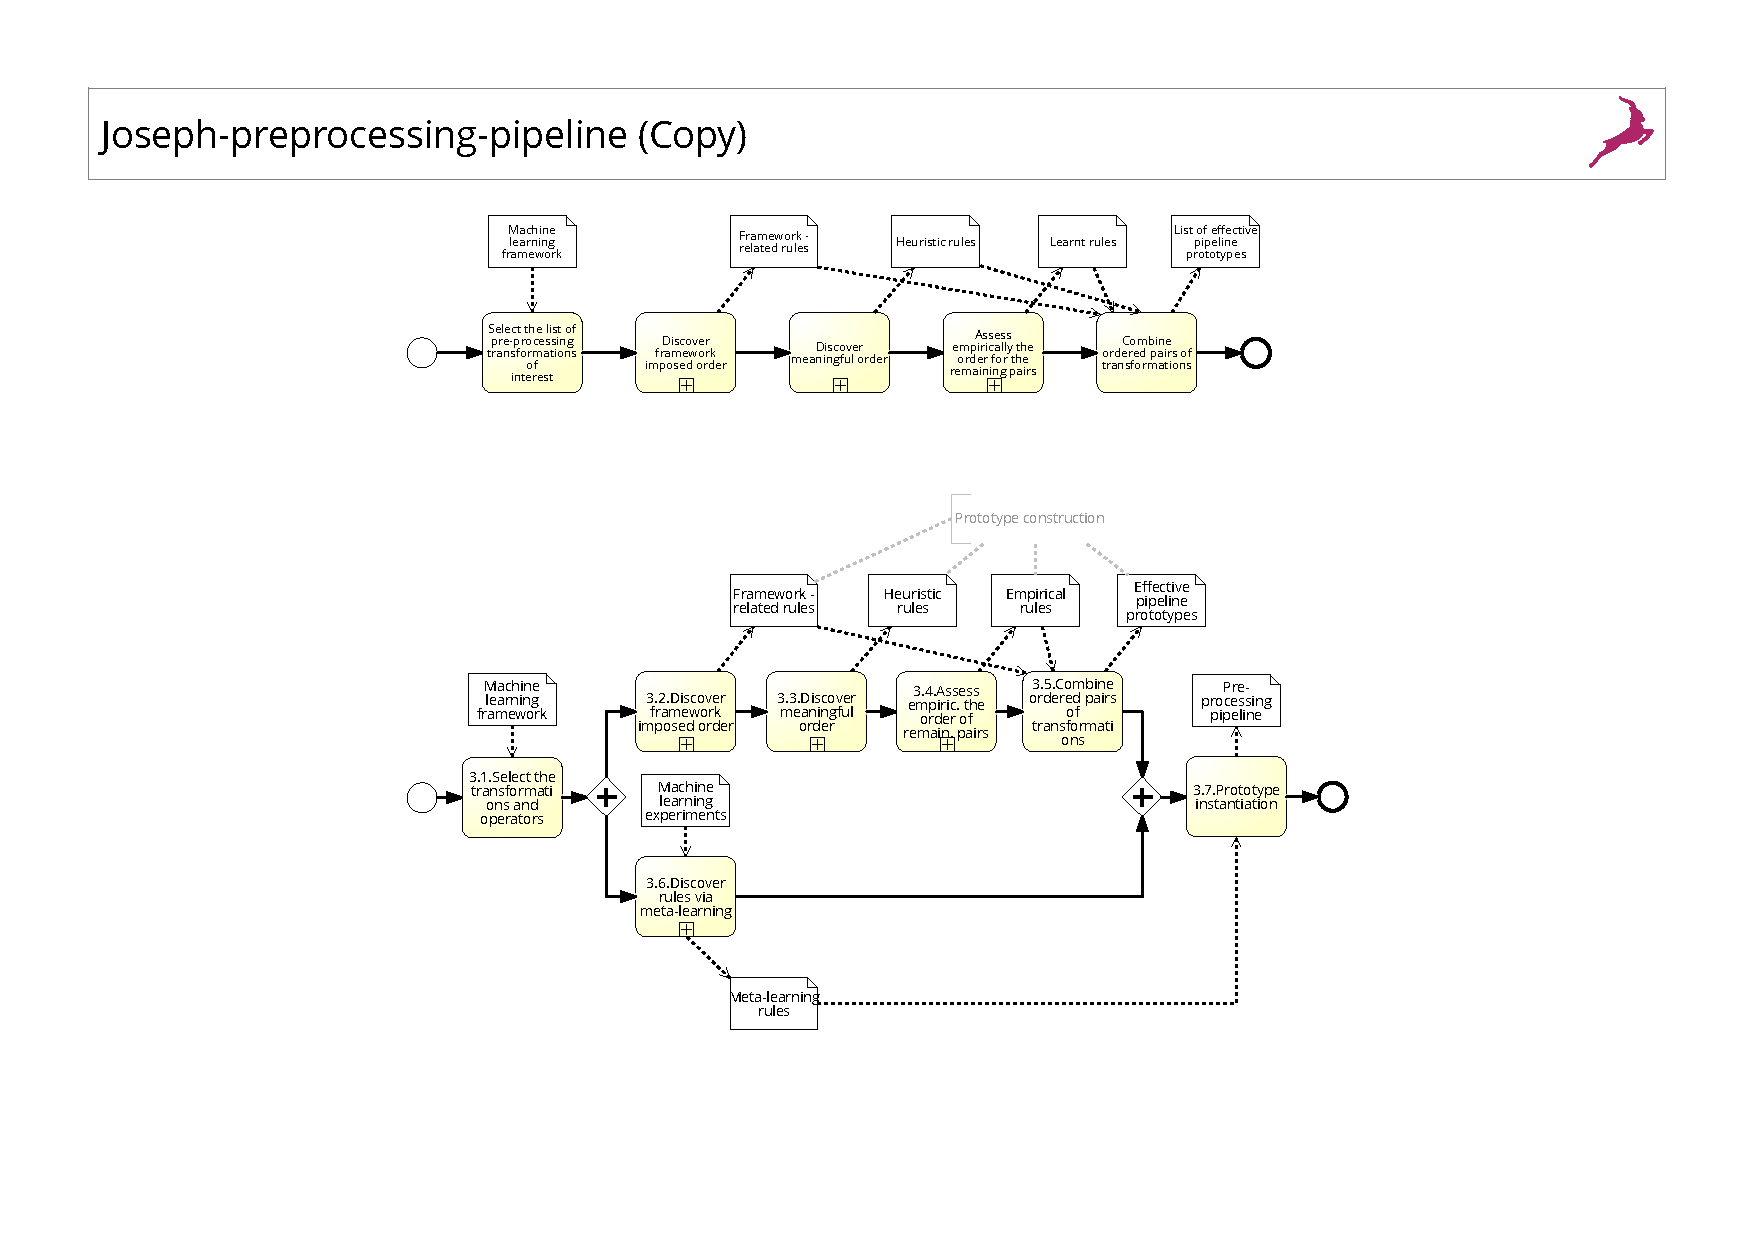
\includegraphics[clip, trim=6.5cm 3.5cm 6.5cm 8cm,width=1.0\textwidth]{part-automl/chapter-supervised/img/bpmn.pdf}
    \caption{A method for generating pre-processing pipelines.}
    \label{fig:methodology}
\end{figure*}

Following the notation from~\cite{Quemy20InfSystems}, we also distinguish between a fixed, ordered sequence of kinds of pre-processing transformations, known as \textit{pipeline prototypes}, and a fixed, ordered sequence of operators (i.e., instantiations of transformations) known as (executable) \textit{pipelines}.
%\textit{pipeline prototype} and a \textit{pipeline}. The former is defined as a fixed, ordered sequence of kinds of pre-processing transformations, where each kind of transformation can be instantiated by a specific set of operators, into an actual executable \textit{pipeline}. 
Typically, pipeline prototype construction is a manual and tedious task, where a data scientist exhaustively iterates over a staggeringly large number of possible pipeline orderings, until he/she finds one that works best for the problem at hand. This is a challenging task due to the fact that there are no clear rules and guidelines in terms of which permutation of kinds of transformations would work best (i.e., the final impact of a pipeline is difficult to foresee). To facilitate it, we propose a method, sketched in Figure~\ref{fig:methodology}, that in short breaks the combinatorial problem of finding the best pipeline into studying kinds of transformations in pairs, ultimately, generating effective pipeline prototypes, which are then fed to an optimizer (e.g., we use the SMBO~\cite{HyperOptICML13} variant), to be instantiated and further optimized.
Some of the steps of the method are generic and thus can be applied regardless of the context, and yet others are specific, and depend on the context (i.e., ML framework used or dataset characteristics).
 
\iffalse
 \besim{To be removed}
%reduce space
\begin{table*}[!t]
\renewcommand{\arraystretch}{0.3}
\footnotesize
\caption{Kinds of transformations and their corresponding operators.}
\centering
\begin{threeparttable}
%\begin{tabular}{@{}ll@{}l|c|c|c|c@{}}
%\subfloat[Framework rules.]{%
\begin{tabular}{@{}p{30mm}lll>{\ttfamily}l@{}}
\toprule
Transf. Kind& Input & Output & Operator & \textnormal{Parameters}
\\	\cmidrule[.1em]{1-5}

Encoding ($E$)  & CA & CO & Ordinal & -  \\ \cmidrule[.05em]{4-5} & & & One Hot & - \\
\cmidrule[.1em]{1-5}

Normalization ($N$) & CO & CO & Standard Scaler & with\_mean:[True,False]\\ \cmidrule[.0em]{4-5}
& & & & with\_std:[True,False] \\ \cmidrule[.05em]{4-5}
&  &  & Power Transform & -\\ \cmidrule[.05em]{4-5}
&  &  & MinMax Scaler & -\\ \cmidrule[.05em]{4-5}
&  &  & Robust Scaler & quantile\_range:[(25,75),(10,90),(5,95)]\\ \cmidrule[.0em]{4-5}
& & & & with\_centering:[True,False]\\ \cmidrule[.0em]{4-5}
& & & & with\_scaling:[True,False] \\ \cmidrule[.1em]{1-5}

Discretization ($D$) & CO & CA & KBins & n\_bins:[3,5,7]\\ \cmidrule[0em]{4-5} 
& & & & encode:[`onehot',`onehot-dense',`ord.']\\ \cmidrule[0em]{4-5} & & & & strategy:[`uniform',`quant.',`kmeans']\\	\cmidrule[.05em]{4-5}
&  &  & Binarization  & threshold: [0, 0.5, 2, 5]\\	\cmidrule[.1em]{1-5}

Imputation ($I$) & CA/CO & CA/CO  & Univariate & strategy:[`most\_freq.','constant'] \\	\cmidrule[.05em]{4-5}
 & &  & Multivariate & initial\_strategy:[`most\_freq',`const.']\\ \cmidrule[0em]{4-5} 
 & & & & order:[`asc',`dsc',`rom',`arab',`rand'] \\	\cmidrule[.1em]{1-5}

Rebalancing ($R$) &CA/CO  & CA/CO & Near Miss & n\_neighbors:[1,2,3]\\ \cmidrule[.05em]{4-5}
&  &  & Condensed KNN & n\_neighbors:[1,2,3] \\ \cmidrule[.05em]{4-5}
&  &  & SMOTE & k\_neighbors:[5,6,7]\\	\cmidrule[.1em]{1-5}

Feat. Eng. ($F$) & CA/CO & CA/CO & PCA & n\_components:[1,2,3,4]\\ \cmidrule[.05em]{4-5}
&  &  & Select K Best & k:[1,2,3,4]\\ \cmidrule[.05em]{4-5}
&  &  & PCA + Select K Best  & n\_components:[1,2,3,4]\\ \cmidrule[0em]{4-5} 
& & & & k:[1,2,3,4]\\	\bottomrule%\cmidrule[.1em]{1-5}
\end{tabular}
\begin{tablenotes}
\footnotesize
\item CA - Categorical, CO - Continuous. 
\end{tablenotes}
\end{threeparttable}
\label{tbl:transformations}
\end{table*}
\fi

The method consists of two flows running in parallel. The first flow is responsible for the pipeline prototype construction and the second flow allows to generate rules that guide the instantiation of the transformations inside the pipeline prototype. 
The output from the two flows is fed to the final step where the instantiation and optimization happens. The result is an executable pipeline. Notice that what we propose is a generic method, however for the sake of an example, we use the OpenML repository~\cite{OpenML2013}, the Scikit-learn library, and the HyperOpt tool, that internally uses SMBO, to provide a use case.

The proposed method starts with the selection of the ML library and optimization framework to be used. On the one hand, this allows to choose the potential kinds of transformations and their available instantiations, and on the other it allows to generate \textit{framework-related rules}, reflecting the limitations in the concrete implementation of operators. These rules enable the generation of precedence relationships between the kinds of transformations for which they apply.
Next, the flow on top continues with a study over all the possible pairs of kinds of transformations, aiming to find the correct/meaningful order between them using \textit{generic knowledge} about their behaviour. As a result, a set of \textit{heuristic rules} that determines precedences between transformations is generated. 
Afterwards, for the pairs for which an order cannot be clearly devised, an additional empirical study is proposed. This study may rely on a testbed of dataset representatives, and thus it may implicitly correspond to \textit{domain knowledge}. The output of this step is a set of \textit{empirically learned rules} that determines promising precedences of transformations (i.e. an order that would potentially positively impact the final result of the analysis). However, even after this phase, for some pairs of transformations a precedence order may not be found. These are pairs for whom the order is relevant but cannot be decided in advance, thus all their permutations need to be present. Finally, a step of composition follows, where given the overall set of devised rules (i.e., \textit{framework-related}, \textit{heuristic} and \textit{empirically learned}), transformations are composed into a set of valid and potentially effective pipeline prototypes. 

Once the prototype is constructed, the flow running in parallel is proposed to help with its instantiation. It consists of a meta-learning step, where a set of ML experiments (e.g., pre-processing and classification algorithm runs) are used as training data, to predict the initial operator for the transformations inside the pipeline prototype. These rules extract knowledge from past experiments and are complementary to the rules obtained in the first flow. They would be used, for example, to ease the cold start problem in the prototype instantiation phase.

\subsubsection{Transformations and Operators}

The first task in the process consists of selecting the kinds of transformations and their available operators. 

When combining two different kinds of transformations, it is important to check if, (i) the input and output types of transformations are compatible, (ii) the combination makes sense, and (iii) the combination provides good results for the analysis. As a result, when chaining a pair of transformations, the following precedence relationships arise:

\begin{enumerate}
    \item Compatible/Incompatible pairs. Depending on whether the representation output of the first transformation is accepted as the representation input of the second one (compatible), or not (incompatible) (see Section~\ref{ssec:rules-framework}).
    \item Meaningful/Meaningless pairs. Depending on whether the precedence between them makes sense based on generic knowledge (i.e., based on the literature) over the behaviour of transformations (meaningful), or not (meaningless) (see Section~\ref{ssec:rules-heuristics}). 
    \item Promising/Unpromising pairs. Depending on whether the precedence between them is expected to provide positive impact on the final result of the analysis (promising), or not (unpromising) (see Section~\ref{ssec:rules-learned}). 
\end{enumerate}

Attending to the relationships between its transformations, a prototype can be described as either \textit{compatible}, \textit{well-formed}, or \textit{effective}. A prototype is defined to be \textit{compatible}, if all its precedence relationships are compatible. It is defined as \textit{well-formed}, if all its precedence relationships are both compatible and meaningful. Finally, it is defined as \textit{effective}, if all its precedence relationships are compatible, meaningful, and promising at the same time. In fact, the ultimate goal of our method is to find \textit{effective pipelines}.

\begin{example}
The kinds of transformations selected for the sake of our use case are the following:

\begin{itemize}[noitemsep,topsep=0pt]
\item{Encoding ($E$).} The process of transforming Categorical attributes into Continuous ones.
\item{Normalization ($N$).} The process of normalizing Continuous attributes such that their values fall in the same range.
\item{Discretization ($D$).} The process of transforming Continuous attributes into Categorical ones.
\item{Imputation ($I$).} The process of imputing missing values.
\item{Rebalancing ($R$).} The process of adjusting the class distribution of a dataset (i.e. the ratio between the different classes/categories represented).
\item{Feature Engineering ($F$).} The process of defining the set of relevant attributes (variables, predictors) to be used in model construction.

\end{itemize}

\begin{table}[!t]
\renewcommand{\arraystretch}{0.3}
\footnotesize
%\caption{Kinds of transformations and their corresponding operators.}
\caption{List of transformations applicable to Categorical or Continuous data types.}
\centering
\begin{threeparttable}
%\begin{tabular}{@{}ll@{}l|c|c|c|c@{}}
%\subfloat[Framework rules.]{%
\begin{tabular}{@{}p{30mm}lll>{\ttfamily}l@{}}
\toprule
Transf. Kind& Input & Output & Operator & \textnormal{Parameters}
\\	\cmidrule[.1em]{1-5}

Encoding ($E$)  & CA & CO & Ordinal & -  \\ \cmidrule[.05em]{4-5} & & & One Hot & - \\
\cmidrule[.1em]{1-5}

Normalization ($N$) & CO & CO & Standard Scaler & with\_mean:[True,False]\\ \cmidrule[]{4-5} & & & & with\_std:[True,False] &  & \\ \cmidrule[.05em]{4-5}
&  &  & Power Transform & -\\ \cmidrule[.05em]{4-5}
&  &  & MinMax Scaler & -\\ \cmidrule[.05em]{4-5}
&  &  & Robust Scaler & quantile\_range:[(25,75),(10,90),(5,95)]\\ \cmidrule[]{4-5} & & & & with\_centering:[True,False]\\ \cmidrule[]{4-5} & & & & with\_scaling:[True,False] \\
\cmidrule[.1em]{1-5}

Discretization ($D$) & CO & CA & KBins & n\_bins:[3,5,7]\\ \cmidrule[]{4-5} & & & & encode:[`onehot',`onehot-dense',`ord.']\\ \cmidrule[]{4-5} & & & & strategy:[`uniform',`quant.',`kmeans']\\	\cmidrule[.05em]{4-5}
&  &  & Binarization  & threshold: [0, 0.5, 2, 5]\\	\cmidrule[.1em]{1-5}

Imputation ($I$) & CA/CO & CA/CO  & Univariate & strategy:[`most\_freq.','constant'] \\	\cmidrule[.05em]{4-5}
 & &  & Multivariate & initial\_strategy:[`most\_freq',`const.']\\ \cmidrule[]{4-5} & & & & order:[`asc',`dsc',`rom',`arab',`rand'] \\	\cmidrule[.1em]{1-5}

Rebalancing ($R$)* &CA/CO  & CA/CO & Near Miss & n\_neighbors:[1,2,3]\\ \cmidrule[.05em]{4-5}
%&  &  & \textcolor{red}{Condensed KNN} & \textcolor{red}{n\_neighbors:[1,2,3]} \\ \cmidrule[.05em]{4-5}
&  &  & SMOTE & k\_neighbors:[5,6,7]\\	\cmidrule[.1em]{1-5}

Feat. Eng. ($F$) & CA/CO & CA/CO & PCA & n\_components:[1,2,3,4]\\ \cmidrule[.05em]{4-5}
&  &  & Select K Best & k:[1,2,3,4]\\ \cmidrule[.05em]{4-5}
&  &  & PCA + Select K Best  & n\_components:[1,2,3,4]
\\ \cmidrule[]{4-5} & & & & k:[1,2,3,4]\\	\bottomrule%\cmidrule[.1em]{1-5}
\end{tabular}
\begin{tablenotes}
\footnotesize
\item CA - Categorical, CO - Continuous. 
\item *All transformations except Rebalancing are taken from scikit-learn.
\end{tablenotes}
\end{threeparttable}
\label{tbl:transformations}
\end{table}

An operator is an actual instantiation/implementation of a kind of transformation. Thus, several operators may implement the same kind of transformation, each having its own set of parameters. For our experiments, we selected the operators and parameters from those available in the Scikit-learn\footnote{\url{https://scikit-learn.org}} library, and they are listed in Table~\ref{tbl:transformations}. \textit{Input} denotes the compatible feature type for a given kind of transformation and can be Continuous (CO) --- when it represents measurements on some continuous scale, or Categorical (CA) --- when it represents information about some categorical or discrete characteristics. Similarly, \textit{Output} denotes the type of the features after a kind of transformation is applied. Finally, \textit{Operator} denotes the physical instantiation for the kind of transformation, and it can be parametrised using its \textit{Parameters}.
\end{example}

%\iffalse
\begin{table*}[!t]
\caption{
    Precedence order between pairs of transformations, represented independently for each phase. 
    }
\renewcommand{\arraystretch}{0.3}
\footnotesize
\begin{center}
%\begin{threeparttable}
%\begin{tabular}{@{}ll@{}l|c|c|c|c@{}}
\subfloat[Compatible precedence.]{%
\begin{tabular}{@{}lcccccc}
\toprule
 & $\boldsymbol{E}$ & $\boldsymbol{N}$ & $\boldsymbol{D}$ & $\boldsymbol{I}$ & $\boldsymbol{R}$ & $\boldsymbol{F}$
\\	\cmidrule[.1em]{1-7}

$\boldsymbol{E}$ & \cellcolor{gray!25} & \texttt{1} & \texttt{1} & \texttt{\texttt{0}} & \texttt{1} & \texttt{1} \\	\cmidrule[.1em]{1-7}
$\boldsymbol{N}$ & \texttt{0} & \cellcolor{gray!25}  & \texttt{0} & \texttt{0} & \texttt{0} & \texttt{0} \\	\cmidrule[.1em]{1-7}
$\boldsymbol{D}$ & \texttt{0} & \texttt{0} & \cellcolor{gray!25}  & \texttt{0} & \texttt{0} & \texttt{0} \\	\cmidrule[.1em]{1-7}
$\boldsymbol{I}$ & \texttt{1} & \texttt{0} & \texttt{1} & \cellcolor{gray!25}  & \texttt{1} & \texttt{1} \\	\cmidrule[.1em]{1-7}
$\boldsymbol{R}$ & \texttt{0} & \texttt{0} & \texttt{0} & \texttt{0} & \cellcolor{gray!25}  & \texttt{0} \\	\cmidrule[.1em]{1-7}
$\boldsymbol{F}$ & \texttt{0} & \texttt{0} & \texttt{0} & \texttt{0} & \texttt{0} & \cellcolor{gray!25}
\\	\bottomrule%\cmidrule[.1em]{1-7}
\end{tabular}}
\qquad% --- set horizontal distance between tables here
\subfloat[Meaningful precedence.]{%
\begin{tabular}{@{}lcccccc}
\toprule
& $\boldsymbol{E}$ & $\boldsymbol{N}$ & $\boldsymbol{D}$ & $\boldsymbol{I}$ & $\boldsymbol{R}$ & $\boldsymbol{F}$
\\	\cmidrule[.1em]{1-7}

$\boldsymbol{E}$ & \cellcolor{gray!25} & \texttt{0} & \texttt{0} & \texttt{0} & \texttt{0} & \texttt{0} \\	\cmidrule[.1em]{1-7}
$\boldsymbol{N}$ & \texttt{0} & \cellcolor{gray!25}  & \texttt{X} & \texttt{0} & \texttt{1} & \texttt{0} \\	\cmidrule[.1em]{1-7}
$\boldsymbol{D}$ & \texttt{0} & \texttt{X} & \cellcolor{gray!25}  & \texttt{0} & \texttt{0} & \texttt{0} \\	\cmidrule[.1em]{1-7}
$\boldsymbol{I}$ & \texttt{1} & \texttt{1} & \texttt{1} & \cellcolor{gray!25}  & \texttt{1} & \texttt{1} \\	\cmidrule[.1em]{1-7}
$\boldsymbol{R}$ & \texttt{0} & \texttt{0} & \texttt{0} & \texttt{0} & \cellcolor{gray!25}  & \texttt{0} \\	\cmidrule[.1em]{1-7}
$\boldsymbol{F}$ & \texttt{0} & \texttt{0} & \texttt{0} & \texttt{0} & \texttt{0} & \cellcolor{gray!25}
\\	\bottomrule%\cmidrule[.1em]{1-7}
\end{tabular}}
\qquad% --- set horizontal distance between tables here
\subfloat[Promising precedence.]{%
\begin{tabular}{@{}lcccccc}
\toprule
& $\boldsymbol{E}$ & $\boldsymbol{N}$ & $\boldsymbol{D}$ & $\boldsymbol{I}$ & $\boldsymbol{R}$ & $\boldsymbol{F}$
\\	\cmidrule[.1em]{1-7}

$\boldsymbol{E}$ & \cellcolor{gray!25} & \texttt{0} & \texttt{0} & \texttt{0} & \texttt{0} & \texttt{0} \\	\cmidrule[.1em]{1-7}
$\boldsymbol{N}$ & \texttt{0} & \cellcolor{gray!25} & \texttt{0} & \texttt{0} & \texttt{0} & \texttt{1} \\	\cmidrule[.1em]{1-7}
$\boldsymbol{D}$ & \texttt{0} & \texttt{0} & \cellcolor{gray!25} & \texttt{0} & \texttt{0} & \texttt{1} \\	\cmidrule[.1em]{1-7}
$\boldsymbol{I}$ & \texttt{0} & \texttt{0} & \texttt{0} & \cellcolor{gray!25} & \texttt{0} & \texttt{0} \\	\cmidrule[.1em]{1-7}
$\boldsymbol{R}$ & \texttt{0} & \texttt{0} & \texttt{0} & \texttt{0} & \cellcolor{gray!25} & \texttt{0} \\	\cmidrule[.1em]{1-7}
$\boldsymbol{F}$ & \texttt{0} & \texttt{0} & \texttt{0} & \texttt{0} & \texttt{0} & \cellcolor{gray!25} 
\\	\bottomrule%\cmidrule[.1em]{1-7}
\end{tabular}}
\end{center}
\begin{tablenotes}
\centering
\scriptsize
\item$\boldsymbol{E}$ - Encoding; $\boldsymbol{N}$ - Normalization; $\boldsymbol{D}$ - Discretization; $\boldsymbol{I}$ - Imputation; $\boldsymbol{R}$ - Rebalancing; $\boldsymbol{F}$ - Feature Engineering. \item \texttt{1} - a precedence edge exists between the row and the column, \texttt{0} - a precedence edge does not exist between the row 
\item and the column, \texttt{X} - the combination is meaningless.
\end{tablenotes}
\label{tbl:rules}
%\end{threeparttable}
\end{table*}

\subsubsection{Framework-related rules}
\label{ssec:rules-framework}
Once the implementation framework is selected, one needs to study it and see if there exist constraints that limit the interaction between transformations. For instance, applying a transformation may actually invalidate the application of another transformation, because the compatibility of transformations is dependent on the selected ML framework.

\begin{example}
We studied the transformations implemented in Scikit-learn and detected a set of implicit rules that are shown through an adjacency matrix, corresponding to a precedence graph, in Table~\ref{tbl:rules}a.
Each cell $a_{ij}$ denotes a precedence relationship between the row $i$ and column $j$. Hence, \texttt{1} means that an edge exists between the transformation in the row and the transformation in the column, whereas \texttt{0} means that such an edge does not exist, hence a precedence order is not established for that pair. 
For example, most Scikit-learn transformations cannot be applied in the presence of missing values. This is why in every pair of transformations where Imputation is involved, except the one with Normalization\footnote{Normalization transformations are the only ones that Scikit-learn can apply on datasets with missing values.}, Imputation goes first.
Furthermore, Scikit-learn transformations are applied only to all compatible attributes of a given dataset. Generally, Categorical attributes are physically represented as strings and Continuous attributes as numbers. However, a transformation that is meant to be applied, say to Continuous attributes, cannot be applied over a dataset that contains both Continuous and Categorical attributes (i.e., a dataset containing both numbers and strings); Scikit-learn cannot deal with arrays of mixed types. In that case, all the Categorical attributes need to be encoded into numeric representations, even if they represent a categorical value. That is, a value can be a number but represent a category. 
This is what happens when Normalization and Discretization are meant to be applied to a dataset containing mixed types of attributes. In order for them to be applied to datasets of mixed types, an Encoding transformation needs to be applied first. A similar constraint is imposed when considering Rebalancing and Feature Engineering, since these transformations do not accept inputs containing strings (i.e., representing a Categorical type). 
For the rest of the pairs of transformations there are no constraints imposed by the framework, thus any order of such transformations is permitted, reflected by a \texttt{0} in Table~\ref{tbl:rules}a.
The graph obtained in this case exclusively corresponds to the limitations of Scikit-learn (as a matter of fact, if another framework were to be chosen, it may have looked differently).
\end{example}

\begin{algorithm*}[b]
	\caption{Find a promising pipeline prototype for transformations $T_1$ and $T_2$}
	\label{alg:learned-rules}
	\begin{algorithmic}[1]
		\REQUIRE $d$, $a$ \COMMENT{dataset, classification algorithm} 
		%\REQUIRE $a$ \COMMENT{classification algorithm}
		\REQUIRE \indent$T_1\rightarrow T_2$, $T_2 \rightarrow T_1$ \COMMENT{precedence orders of a pair of transformations}
		\STATE $acc_{baseline} = Acc(d,a)$; \COMMENT{get baseline performance of algorithm on d}
		\STATE $[pipeline_{T_1\rightarrow T_2},acc_{T_1\rightarrow T_2}] = SMBO(T_1\rightarrow T_2,d, a)$ 
		
		\COMMENT{get pipeline and accuracy for $T_1\rightarrow T_2$}
		\STATE $[pipeline_{T_2\rightarrow T_1},acc_{T_2\rightarrow T_1}] = SMBO(T_2\rightarrow T_1,d, a)$
		
		\COMMENT{get pipeline and accuracy for $T_2\rightarrow T_1$}
		\IF[see Table~\ref{tbl:validation-rules} for the rules applied]{\textit{IsValid}($acc_{T_1\rightarrow T_2},acc_{T_2\rightarrow T_1},acc_{baseline}$)}
		\RETURN \textit{Winner}$([pipeline_{T_1\rightarrow T_2},acc_{T_1\rightarrow T_2}],[pipeline_{T_2\rightarrow T_1},acc_{T_2\rightarrow T_1}])$ 
		
		\COMMENT{see column \textit{Winner prototype} in Table~\ref{tbl:validation-rules}}
		\ELSE
		\RETURN $\varnothing$
		\ENDIF
	\end{algorithmic}
\end{algorithm*}

\subsubsection{Heuristic rules}
\label{ssec:rules-heuristics}
In the previous section, we proposed to derive a precedence based on the constraints of the framework. Now, we want to study the precedence independently of the framework, and find \textit{meaningful pairs}. That is, for every given pair, we want to find the relative order, based on generic, domain-independent knowledge (i.e., literature) about transformations and their applicability. To this end, some of the constraints imposed by the framework may be contradicted here, but this is resolved in the last step of the proposed method, when we take the union of the rules and hence construct the final pipeline prototypes (see Section~\ref{ssec:composition}). Briefly, in a combination where Imputation is involved, it is advised to apply Imputation first. Next, an Encoding transformation makes sense to be combined in any order with the rest of transformations, except Imputation. 
Combining Discretization with Normalization does not make sense, due to the fact that after the Discretization step, Continuous attributes are transformed into Categorical ones, and hence Normalization cannot be applied. Similarly, applying Normalization first, changes the scale of the values and hence impacts the Discretization step. Finally, a meaningful precedence can be derived when combining Normalization with Rebalancing. In this case, Normalization should be applied first, since otherwise Rebalancing would impact the scale of the values to be normalized.

\begin{example}
For our use case, Table~\ref{tbl:rules}b shows the heuristic rules obtained considering domain-independent knowledge about transformations~\cite{BookExploratoryDM03Dasu}. In comparison with the results from Table~\ref{tbl:rules}a, observe that the constraints on the Imputation transformation still hold, that is, it is correct to apply Imputation first when combining it with another transformation. This time even when combining it with Normalization --- note the difference with Table~\ref{tbl:rules}a. The constraints of Encoding are however not present in Table~\ref{tbl:rules}a, hence not considering the framework, Discretization combined with Encoding is a meaningful combination --- when a mixed type dataset is considered, but incompatible from the point of view of Scikit-learn.
\end{example}

\subsubsection{Empirically learned rules}
\label{ssec:rules-learned}

The two previously proposed steps (i.e., \textit{framework-related} and \textit{heuristic rules}), do not guarantee that for each pair of transformations we will obtain a precedence order. Therefore, for the cases where they are not sufficient to determine the precedence, a third viewpoint can be considered. That of learning a promising order by empirically studying the impact of the combinations on the final result of the analysis, using different classification problems in the training. For every selected pair of transformations, for a given classification algorithm, we propose to check which order of the pair improves most the performance (e.g., predictive accuracy) of the algorithm over a set of datasets (preferably from different domains). Like this, for each dataset we can get a precedence order that gives better results (i.e., promising precedence) in terms of predictive accuracy (other metrics can be used as well). 

\paragraph{Algorithm}
\label{ssec:rules-learned:algorithm}

\begin{table*}[t]
%\renewcommand{\arraystretch}{0.3}
\footnotesize
\centering
\begin{threeparttable}
\caption{
    Validation rules.
    }
%\begin{tabular}{@{}ll@{}l|c|c|c|c@{}}
%\subfloat[Framework rules.]{%
\begin{tabular}{@{}lllllc@{}}
\toprule
Nr. & Pipeline 1 & Pipeline 2 & Valid result & Valid score & Winner prototype\\\toprule
         1. &$\varnothing \rightarrow \varnothing$ & $\varnothing \rightarrow \varnothing$ & Draw          & $acc_{baseline}$ &  Baseline \\ \hline
        2. &$\varnothing \rightarrow \varnothing$ & $con\!f_{T_2} \rightarrow \varnothing$ & Draw          & $acc_{baseline}$ & Baseline \\ \hline
        3. &$\varnothing \rightarrow \varnothing$ & $\varnothing \rightarrow con\!f_{T_1}$ & Draw          & $acc_{baseline}$ & Baseline \\ \hline
        \multirow{2}{*}{4.} &\multirow{2}{*}{$\varnothing \rightarrow \varnothing$} & \multirow{2}{*}{$con\!f_{T_2} \rightarrow con\!f_{T_1}$} & Draw & $acc_{baseline}$ & Baseline \\
        & & & $con\!f_{T_2} \rightarrow con\!f_{T_1}$ & $acc_{T_2 \rightarrow  T_1}$ & $T_2 \rightarrow T_1$\\ \hline
        
        5. & $\varnothing \rightarrow con\!f_{T_2}$ & $\varnothing \rightarrow \varnothing$ & Draw          & $acc_{baseline}$ & Baseline \\ \hline
        \multirow{3}{*}{6.} & \multirow{3}{*}{$\varnothing \rightarrow con\!f_{T_2}$} & \multirow{3}{*}{$con\!f_{T_2} \rightarrow \varnothing$} & Draw &  \multirow{3}{*}{$acc_{T_2}$}  & $T_2$ \\
        & & & $\varnothing \rightarrow con\!f_{T_2}$ & & $T_2$ \\
        & & & $con\!f_{T_2} \rightarrow \varnothing$ & & $T_2$ \\ \hline
        7. &$\varnothing \rightarrow con\!f_{T_2}$ & $\varnothing \rightarrow con\!f_{T_1}$ & Draw & $acc_{T_2}$ or $acc_{T_1}$ & $T_{1}\,or\, T_2$ \\ \hline
        \multirow{2}{*}{8.} & \multirow{2}{*}{$\varnothing \rightarrow con\!f_{T_2}$} & \multirow{2}{*}{$con\!f_{T_2} \rightarrow con\!f_{T_1}$} & Draw & $acc_{T_2}$ & $T_2$\\
        & & & $con\!f_{T_2} \rightarrow con\!f_{T_1}$ & $acc_{T_2 \rightarrow  T_1}$ & $T_2 \rightarrow T_1$ \\ \hline
        
        9. & $con\!f_{T_1} \rightarrow \varnothing$ & $\varnothing \rightarrow \varnothing$ & Draw & $acc_{baseline}$ & Baseline \\ \hline
        10. & $con\!f_{T_1} \rightarrow \varnothing$ & $con\!f_{T_2} \rightarrow \varnothing$ & Draw & $acc_{T_1}$ or $acc_{T_2}$ & $T_{1}\,or\, T_2$ \\ \hline
        \multirow{3}{*}{11.} & \multirow{3}{*}{$con\!f_{T_1} \rightarrow \varnothing$} & \multirow{3}{*}{$\varnothing \rightarrow con\!f_{T_1}$} & Draw & \multirow{3}{*}{$acc_{T_1}$} & $T_1$\\
        & & & $con\!f_{T_1} \rightarrow \varnothing$ & & $T_1$\\
        & & & $\varnothing \rightarrow con\!f_{T_1}$ & & $T_1$\\ \hline
        \multirow{2}{*}{12.} & \multirow{2}{*}{$con\!f_{T_1} \rightarrow \varnothing$} & \multirow{2}{*}{$con\!f_{T_2} \rightarrow con\!f_{T_1}$} & Draw & $acc_{T_1}$  & $T_1$\\
        & & & $con\!f_{T_2} \rightarrow con\!f_{T_1}$ & $acc_{T_2 \rightarrow  T_1}$ & $T_2 \rightarrow T_1$ \\ \hline
        
        \multirow{2}{*}{13.} & \multirow{2}{*}{$con\!f_{T_1} \rightarrow con\!f_{T_2}$} & \multirow{2}{*}{$\varnothing \rightarrow \varnothing$} & Draw & $acc_{baseline}$  & Baseline\\
        & & & $con\!f_{T_1} \rightarrow con\!f_{T_2}$ & $acc_{T_1 \rightarrow  T_2}$ & $T_1 \rightarrow T_2$ \\ \hline
        \multirow{2}{*}{14.} & \multirow{2}{*}{$con\!f_{T_1} \rightarrow con\!f_{T_2}$} & \multirow{2}{*}{$con\!f_{T_2} \rightarrow \varnothing$} & Draw & $acc_{T_2}$ & $T_2$\\
        & & & $con\!f_{T_1} \rightarrow con\!f_{T_2}$ & $acc_{T_1 \rightarrow  T_2}$  & $T_1 \rightarrow T_2$ \\ \hline
        \multirow{2}{*}{15.} & \multirow{2}{*}{$con\!f_{T_1} \rightarrow con\!f_{T_2}$} & \multirow{2}{*}{$\varnothing \rightarrow con\!f_{T_1}$} & Draw & $acc_{T_1}$ & $T_1$\\
        & & & $con\!f_{T_1} \rightarrow con\!f_{T_1}$ & $acc_{T_1 \rightarrow  T_2}$ & $T_1 \rightarrow T_2$\\ \hline
        \multirow{3}{*}{16.} & \multirow{3}{*}{$con\!f_{T_1} \rightarrow con\!f_{T_2}$} & \multirow{3}{*}{$con\!f_{T_2} \rightarrow con\!f_{T_1}$} & Draw & $acc_{T_1}$ or $acc_{T_2}$ & $T_{1}\,or\, T_2$ \\
        & & & $con\!f_{T_1} \rightarrow con\!f_{T_2}$ & $acc_{T_1 \rightarrow  T_2}$ & $T_1 \rightarrow T_2$\\
        & & & $con\!f_{T_2} \rightarrow con\!f_{T_1}$ & $acc_{T_2 \rightarrow  T_1}$ & $T_2 \rightarrow T_1$\\ \bottomrule
\end{tabular}
\begin{tablenotes}
\footnotesize
\item $\varnothing$ - SMBO finds a better result without instantiating a transformation (or both) in the pair.
%None, in case where SMBO finds a better result without instantiating a transformation (or both) in the pair.
\item $con\!f_T$ - The configuration (i.e., operator and its parameters) found for $T$ by SMBO.
\item $acc_T$ - The accuracy of the ML algorithm over the data transformed with a pipeline $T$.
\end{tablenotes}
    \label{tbl:validation-rules}
\end{threeparttable}
\end{table*}

\begin{figure*}[!b]
	\centering
	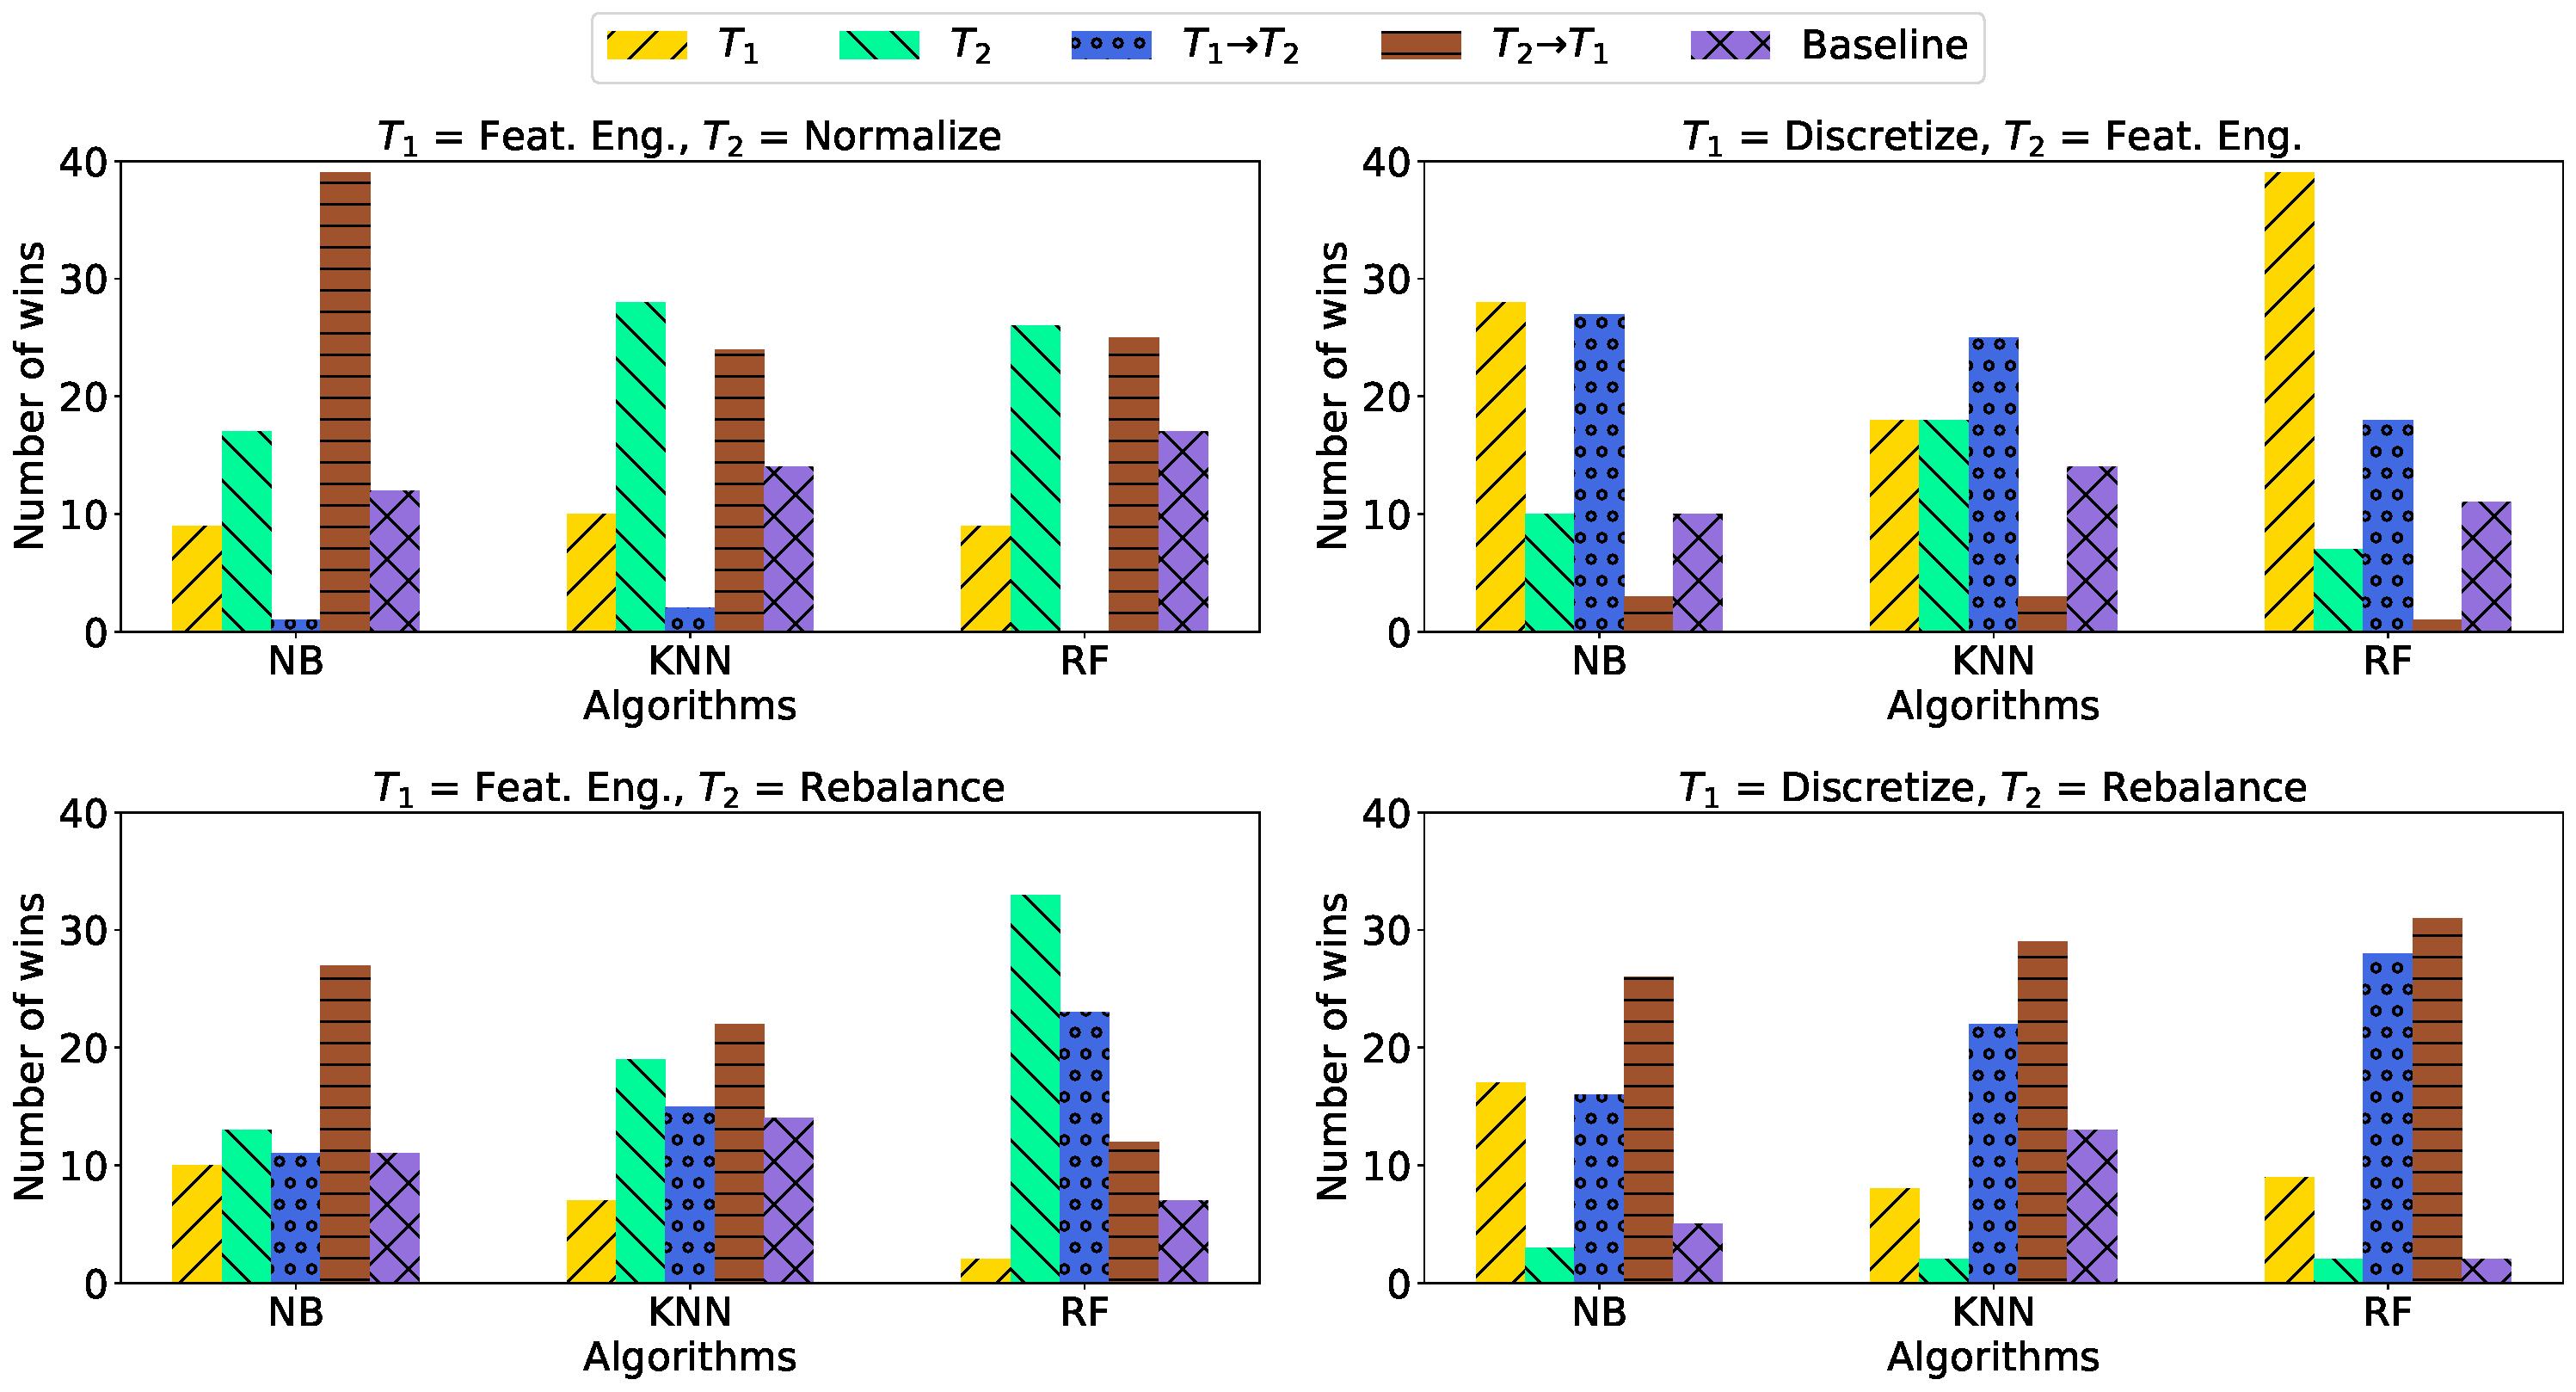
\includegraphics[width=1.0\textwidth]{part-automl/chapter-supervised/img/experiments_results.pdf}
	\caption{Number of datasets for which a given pipeline prototype is declared the winner.}
	\label{fig:learned-rules-results}
\end{figure*}

To find a promising precedence order between a given pair of transformations, we propose Algorithm~\ref{alg:learned-rules}. 
To compute the impact of transformations, we first get the accuracy of the ML algorithm over the original non-transformed dataset (see line 1). %, which is used later for calculating the change in accuracy. 
Afterwards, for each precedence order between the pairs of transformations, we find both their optimized executable pipelines (i.e., using SMBO), and the accuracies of the ML algorithm (with default parametrisation) over the datasets transformed using the respective pipelines (see lines 2-3). Based on the comparison between the respective optimized pipelines, we get the winner in line 5. However, beforehand, in line 4, we perform a validity check. This is because when optimizing a pre-processing pipeline, SMBO may not instantiate a transformation with an operator at all (i.e., represented with a $\varnothing$ symbol).
Hence, given a pair of transformations, where one or both of them may not be instantiated, SMBO may generate 16 possible scenarios. They are listed in Table~\ref{tbl:validation-rules}, and make up the validation rules for Algorithm~\ref{alg:learned-rules} (see line 4). 

Briefly, if among the optimized pairs of transformations (same transformations but in reverse order) obtained from SMBO, one or both of them contain a $\varnothing$ operator, their results are considered valid, only if they have equal scores (i.e., a draw). This is because, if one has a higher score, it means that during the optimization phase it was more advantageous than the other, since it could find a configuration that should have been found by both of the pairs, given enough budget. In our SMBO runs, such invalid results account for less than 10\% and in those cases datasets are discarded from the study (see line 7). 

In particular, in Table~\ref{tbl:validation-rules}, the first two columns denote the pipeline instantiations for the respective pairs of transformations (i.e., $T_1\rightarrow T_2$ and $T_2\rightarrow T_1$). Next, \textit{Valid result} denotes the expected result when comparing the results of the pipelines in the same row. For instance, in the first row, if both transformations in the pipelines are not instantiated during the optimization, a valid result is a draw, and a \textit{Valid score} for the respective result is the baseline accuracy, and the \textit{Winner prototype} is the prototype that is in accordance with the expected result, which in this case is the Baseline (i.e., prototype consisting of only the ML algorithm, where no transformations are applied).

%achieves a valid result, which is the baseline in our example.
For the sake of another example, let us check row 2 in Table~\ref{tbl:validation-rules}. Running SMBO, the best result for the first pair is the pipeline $\varnothing \rightarrow \varnothing$, and for the second pair, the pipeline $T_2 \rightarrow \varnothing$. In this case, the comparison between the results of these pipelines should be equal (i.e., draw), and the score should be that of the baseline. Otherwise, if say, the score of the second pipeline was higher, it would mean that for the first pair, SMBO was not given enough time to find the pipeline with higher score (i.e., $T_2\rightarrow \varnothing$).
The same logic applies also for the other rows where a $\varnothing$ operator is involved.

\color{black}

%\subsubsection{\textcolor{blue}{Use Case: Empirically learnt rules}}
\begin{example}
%\joseph{I added the OpenMLCC18 benchmark link, is that okay?}
For the sake of this work, we considered three classification algorithms (i.e., \textit{NB}, \textit{RF},  \textit{KNN}) and 80 datasets from the OpenML repository. The datasets, were compiled from three OpenML benchmarks, namely, the OpenMLCC18 benchmark\footnote{\url{https://www.openml.org/s/99/data}}, the AutoML benchmark\footnote{\url{https://www.openml.org/s/271/data}}, and the Classification algorithms benchmark\footnote{\url{https://www.openml.org/s/1/data}}. For the final set, we filtered out datasets with more than 10\% of missing values --- not to include bias due to the heavy pre-processing we need to perform on top of them, and we filtered out the datasets with more than 5 million instances --- because of the computation time required to process them. As a result we obtained 60 datasets from the first benchmark, 17 from the second, and 3 more from the third to reach a total of 80 datasets. 

Given the proposed algorithm (i.e. Algorithm~\ref{alg:learned-rules}), we could try to learn the precedence of every pair of transformations, but would just be a waste of resources, because we can see in Table~\ref{tbl:rules}a and~\ref{tbl:rules}b, that some precedences are already decided for one reason or another. Hence, only pairs of transformations with a \texttt{0} for both directions (in both Table~\ref{tbl:rules}a and~\ref{tbl:rules}b) need to be studied further. That is, they make sense to be combined together, but a precedence order could not be determined through \textit{framework-related} or \textit{heuristic rules}. % for them. 
Thus, for instance, pairs involving Encoding are not considered in this phase, since for them an order is already imposed by the framework (see Table~\ref{tbl:rules}a).
To this end, the pairs of transformations we consider for the third precedence graph include only $\{F,N\}$, $\{F,D\}$, $\{F,R\}$, and $\{R,D\}$.

\begin{table}[t]
	\centering
	\footnotesize
	\begin{threeparttable}
		\caption{
			Binomial test for determining the order between pairs of transformations. 
		}
		\label{tbl:significance-test}
		\begin{tabular}{@{}cccccc@{}}
			\toprule
			%$T_1$ & $T_2$ & $T_1 \rightarrow T_2$ & $T_2 \rightarrow T_1$ & alpha & \begin{tabular}[c]{@{}c@{}}p-value\\ $H_0:\pi = \pi_0=0.8$\end{tabular} \\ \midrule
			$T_1$ & $T_2$ & $T_1 \rightarrow T_2$ & $T_2 \rightarrow T_1$ & alpha & p-value\\ \midrule
			$F$ & $N$ & 3 & 88 & 0.05 &  \textbf{0} \\
			$D$ & $F$ & 70 & 7 & 0.05 &  \textbf{0}  \\
			$F$ & $R$ & 49 & 61 & 0.05 & 8.53e-01 \\
			$D$ & $R$ & 66 & 86 & 0.05 & 9.38e-01 \\ \bottomrule
		\end{tabular}
		\begin{tablenotes}
		\centering
		\scriptsize
		\item$N$ - Normalization; $D$ - Discretization; $R$ - Rebalancing; $F$ - Feature Engineering. 
		\end{tablenotes}
	\end{threeparttable}
\end{table}
Applying Algorithm~\ref{alg:learned-rules}, we obtain a pro\-mising order for each pair of transformations considered. %(i.e., $\{F,N\}$, $\{F,D\}$, $\{F,R\}$, $\{R,D\}$). 
Since SMBO is a randomized algorithm we experimented with (i) running it several times splitting the budget, and (ii) running it only once with the entire budget. For the experiments considered, no significant differences where observed, therefore we opted for running it once with the entire budget (i.e., 200 seconds per run), which allows for more configurations to be visited in a single run. Aggregating all the results, Figure~\ref{fig:learned-rules-results} shows the number of datasets, for which a given prototype (see Table~\ref{tbl:validation-rules}, column \textit{Winner prototype} for the list of labels) is selected as the winner. For instance, for the pair $\{F,N\}$ (i.e., Feature Engineering, Normalization), the prototype winning in more datasets for \textit{KNN} and \textit{NB} is $N\rightarrow F$. This means that in general, better results are obtained if Normalization is applied before Feature Engineering. 

Next, only $N$ appears as first for \textit{RF} and second best for \textit{KNN} and \textit{NB}, which means that for many datasets, considering different algorithms, it results better to apply only Normalization without combining it with Feature Engineering. The third position is for $\varnothing\rightarrow \varnothing$, which means that for some datasets it is better not to apply any of the transformations (in any combination). The remaining prototypes winning in some datasets are $F$ (only Feature Engineering), and $F \rightarrow N$ (Feature Engineering preceding Normalization).  Finally, for three datasets, that are omitted from the figure, there were no winning pipelines (i.e., pipelines resulted in a draw).

Since our goal is to find the best order for a pair of transformations, we focus on the performances of the pipelines where both of the transformations are instantiated (i.e., $T_1\rightarrow T_2$ versus $T_2\rightarrow T_1$). To do this, we check whether the difference between the number of datasets where they each appear to win are statistically significant by running a binomial test assuming a theoretical probability of 0.5. The results are shown in Table~\ref{tbl:significance-test}.
In summary, the results from Table~\ref{tbl:significance-test} indicate that, with 95\% confidence we can assume that for the pair $\{F,N\}$, $N\rightarrow F$ performs better than $F\rightarrow N$, hence Normalization should precede Feature Engineering. On the other hand, for $\{D,F\}$, $D\rightarrow F$ performs better than $F\rightarrow D$, hence Discretization should precede Feature Engineering. Finally, for the remaining transformations, $\{F,R\}$ and $\{R,D\}$, a precedence order can not be pre-assumed since the results obtained are not significant. 
Using these results, we create the \textit{Promising precedence} adjacency matrix shown in Table~\ref{tbl:rules}c, where as one can observe, precedence edges are introduced for $\{N,F\}$ and $\{D,F\}$, but no edges exist neither for $\{F,R\}$, nor for $\{R,D\}$. 
\end{example}

\paragraph{Cross-validation}
\label{ssec:learned-rules-validation}
After running Algorithm~\ref{alg:learned-rules} to empirically find a winner between two pairs of transformations, we may obtain a different distribution of the number of wins for the pairs, depending on the datasets considered. To show that the results obtained with the initial set of datasets are generalizable, we propose to perform an additional cross-validated experiment, where the set of datasets considered can be randomly split into many folds. Then, for each fold, the results can be compared to the rest, with the aim of checking whether the distributions are similar. This check can be done via a significance test (e.g., chi-square). To this end, if the distributions between the folds are similar, it means that the obtained results are independent of the datasets considered, since no matter the combination of the datasets, the results are the same and thus generalizable.


%To further validate the results and show that they do not depend on the datasets selected, we re-run the experiments (i.e., 10-times each), but this time splitting the datasets into 4-folds. We wanted to check if the results of the precedence orders from the different folds (i.e., for each experiment considering a randomly different set of datasets) are similar between them (i.e., follow the same distributions). If they are similar, it means that the obtained results are independent of the datasets considered, since no matter the combination of datasets, the results are the same.
\color{black}

\begin{example}
In our use case, to show that the results do not depend on the datasests selected, we re-run the experiments (i.e., 10-times each), but this time splitting the datasets into 4-folds. The goal was to check if the results of the precedence orders from the different folds (i.e., for each experiment considering a randomly different set of datasets) are similar between them (i.e., follow the same distributions).
To confirm this hypothesis, we perform a chi-square test between the results (precedence orders) obtained in a single fold in comparison to the three remaining folds, hence comparing 25\% of the datasets to the rest. 
%In contrast to the previous case of Figure~\ref{fig:learned-rules-results}, where the null hypothesis was that ``the precedence orders follow the same distribution" (we were comparing $T_1\rightarrow T_2$ against $T_2\rightarrow T_1$), and we rejected it by looking at the p-value and finding it less than 0.05 (sticking to 95\% confidence), in this case, our null-hypothesis is ``the precedence orders of the different folds follow the same distribution", but looking at the p-values we find that they are all higher than 0.05. Hence, the higher the p-value, the further we are from rejecting the null-hypothesis, thus the more similar are the results between the folds.
%\textcolor{red}{We recall that, in the previous case (Figure~\ref{fig:learned-rules-results}), we exploited such a test to compare the distribution resulting from the experiments (consisted by the frequencies of $T_1\rightarrow T_2$ and $T_2\rightarrow T_1$) with the uniform distribution. 
%The more they differ, the greater the validity of the created \textit{Promising precedence}. 
%\besim{Do you refer here to the previous binomial test? I think we don't have to refer to the previous test.}
%Since the null hypothesis always claims ``there is no significant difference between the two distributions", and our aim is to reject it, we sought for p-values less than 0.05 (95\% of confidence). Conversely, in this case, we want to assure that the distributions resulting from the different folds do not differ. Thus, by sticking with a 95\% of confidence, we seek for p-values greater than 0.05 to accept the null-hypothesis. 
%The higher the p-value, the further we are from rejecting the null-hypothesis, thus the more similar are the results between the folds.Looking at the p-values we find that they are all higher than 0.05.
%Specifically,}
%\besim{An alternative to the two red paragraphs above:}
In particular, to confirm the hypothesis, we need to find results that accept the null hypothesis of the chi-square test which states that "there is no significant difference between the distributions". To do that, sticking to the 95\% confidence interval, we need to look for p-values greater than 0.05. That is, the higher the p-values, the more we accept the null hypothesis, the more similar the distributions. Looking at the p-values we found out that they were all much higher than 0.05. Specifically, the scores of the chi-square tests of the folds (one fold compared to the rest) are averaged and, after having repeated this procedure 10 times, instead of using a table we depict the 10 averaged p-values using box-plots in Figure~\ref{fig:10-times-4-cv}.
We conclude that, for both of the rules (i.e.,  $F\rightarrow N$ and $F\rightarrow D$), the significance test indicates a compliance between the new results (Figure~\ref{fig:10-times-4-cv}) and those illustrated above (Table~\ref{tbl:significance-test}).



\begin{figure*}[!t]
	\centering
	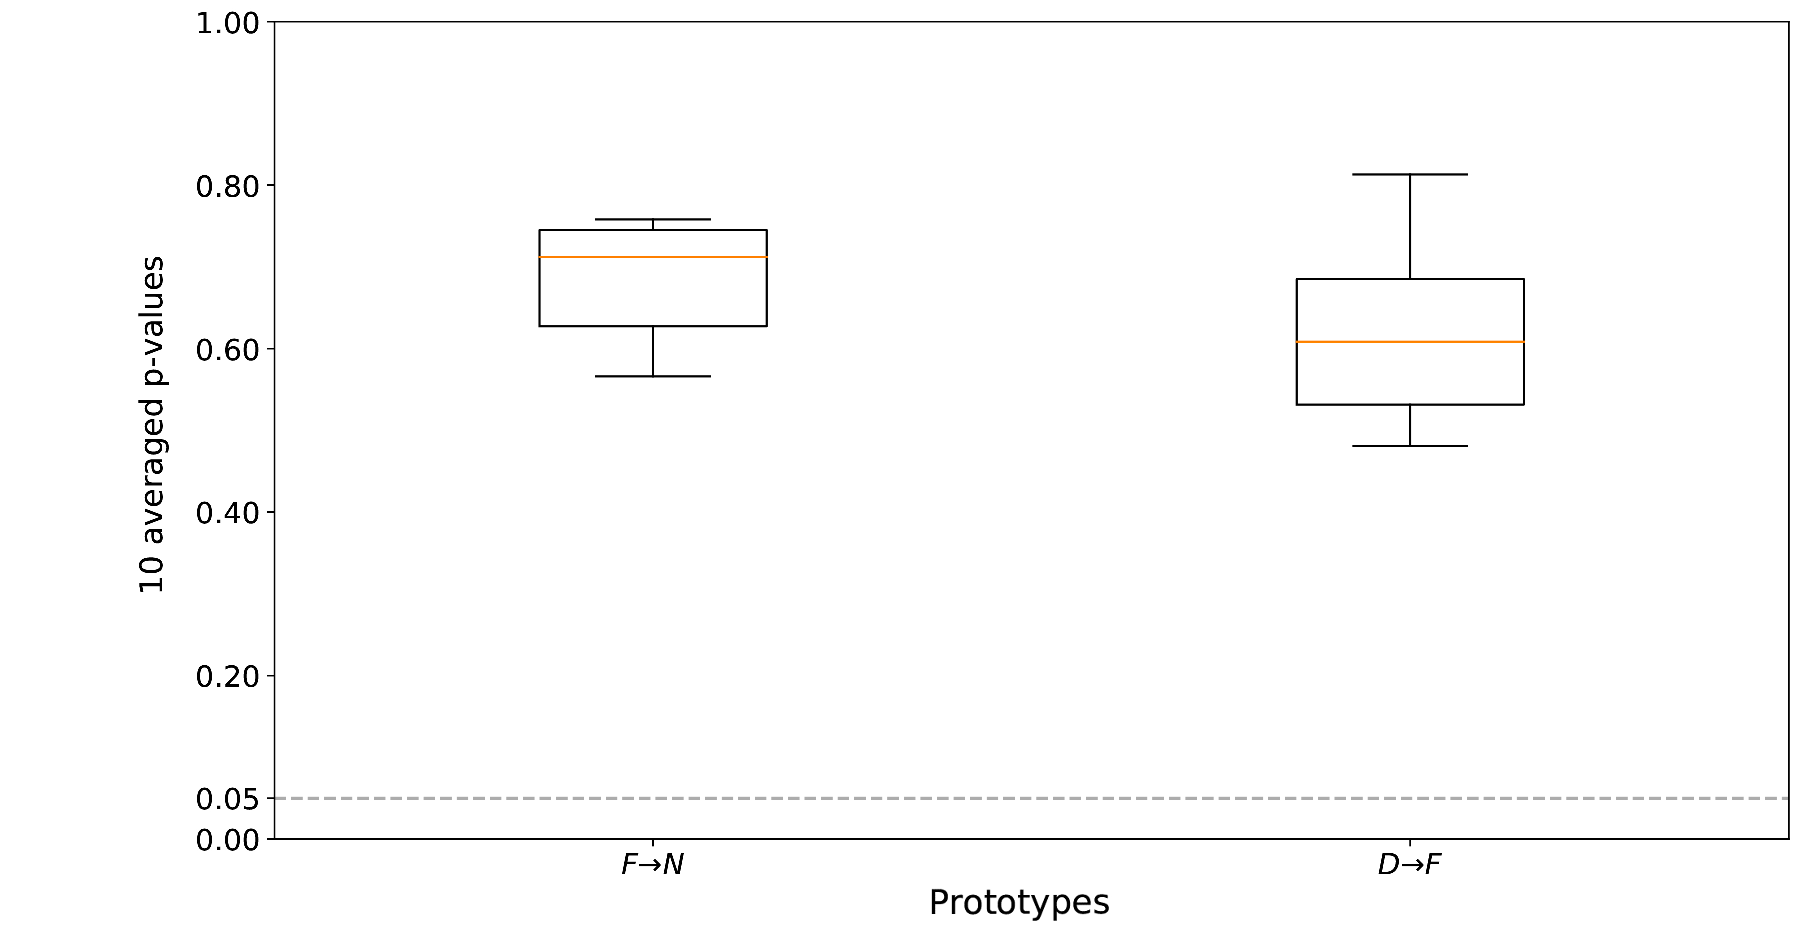
\includegraphics[width=0.9\textwidth]{part-automl/chapter-supervised/img/10_times_4_folds_cv.pdf}
	\caption{The distribution of the p-values obtained after repeating the chi-square test for 10 times, for the 10 times 4-fold cross-validation.}
	\label{fig:10-times-4-cv}
	%\alberto{10 averaged p-values?}
\end{figure*}

\begin{table}[b]
	\caption{
		Union of rules from Table~\ref{tbl:rules}. $\boldsymbol{E}$ - Encoding; $\boldsymbol{N}$ - Normalization; $\boldsymbol{D}$ - Discretization; $\boldsymbol{I}$ - Imputation; $\boldsymbol{R}$ - Rebalancing; $\boldsymbol{F}$ - Feature Engineering \texttt{1} - an edge exists, \texttt{0} - edge does not exist, \texttt{X} - the combination is meaningless.
	}
	\renewcommand{\arraystretch}{0.3}
	\footnotesize
	\centering
	\label{tbl:rules-union}
	\begin{threeparttable}
		%\begin{tabular}{@{}ll@{}l|c|c|c|c@{}}
		\begin{tabular}{@{}lcccccc}
			\toprule
			& $\boldsymbol{E}$ & $\boldsymbol{N}$ & $\boldsymbol{D}$ & $\boldsymbol{I}$ & $\boldsymbol{R}$ & $\boldsymbol{F}$
			\\	\cmidrule[.1em]{1-7}
			$\boldsymbol{E}$ & \cellcolor{gray!25} & \texttt{1} & \texttt{1} & \texttt{0} & \texttt{1} & \texttt{1} \\	\cmidrule[.1em]{1-7}
			$\boldsymbol{N}$ & \texttt{0} & \cellcolor{gray!25}  & \texttt{X} & \texttt{0} & \texttt{1} & \texttt{1} \\	\cmidrule[.1em]{1-7}
			$\boldsymbol{D}$ & \texttt{0} & \texttt{X} & \cellcolor{gray!25} & \texttt{0} & \texttt{0} & \texttt{1} \\	\cmidrule[.1em]{1-7}
			$\boldsymbol{I}$ & \texttt{1} & \texttt{1} & \texttt{1} & \cellcolor{gray!25}  & \texttt{1} & \texttt{1} \\	\cmidrule[.1em]{1-7}
			$\boldsymbol{R}$ & \texttt{0} & \texttt{0} & \texttt{0} & \texttt{0} & \cellcolor{gray!25}  & \texttt{0} \\	\cmidrule[.1em]{1-7}
			$\boldsymbol{F}$ & \texttt{0} & \texttt{0} & \texttt{0} & \texttt{0} & \texttt{0} & \cellcolor{gray!25} \\	\cmidrule[.1em]{1-7}
		\end{tabular}
	\end{threeparttable}
\end{table}

\begin{figure}
\begin{floatrow}
\ffigbox{%
	%left, lower, right, upper
    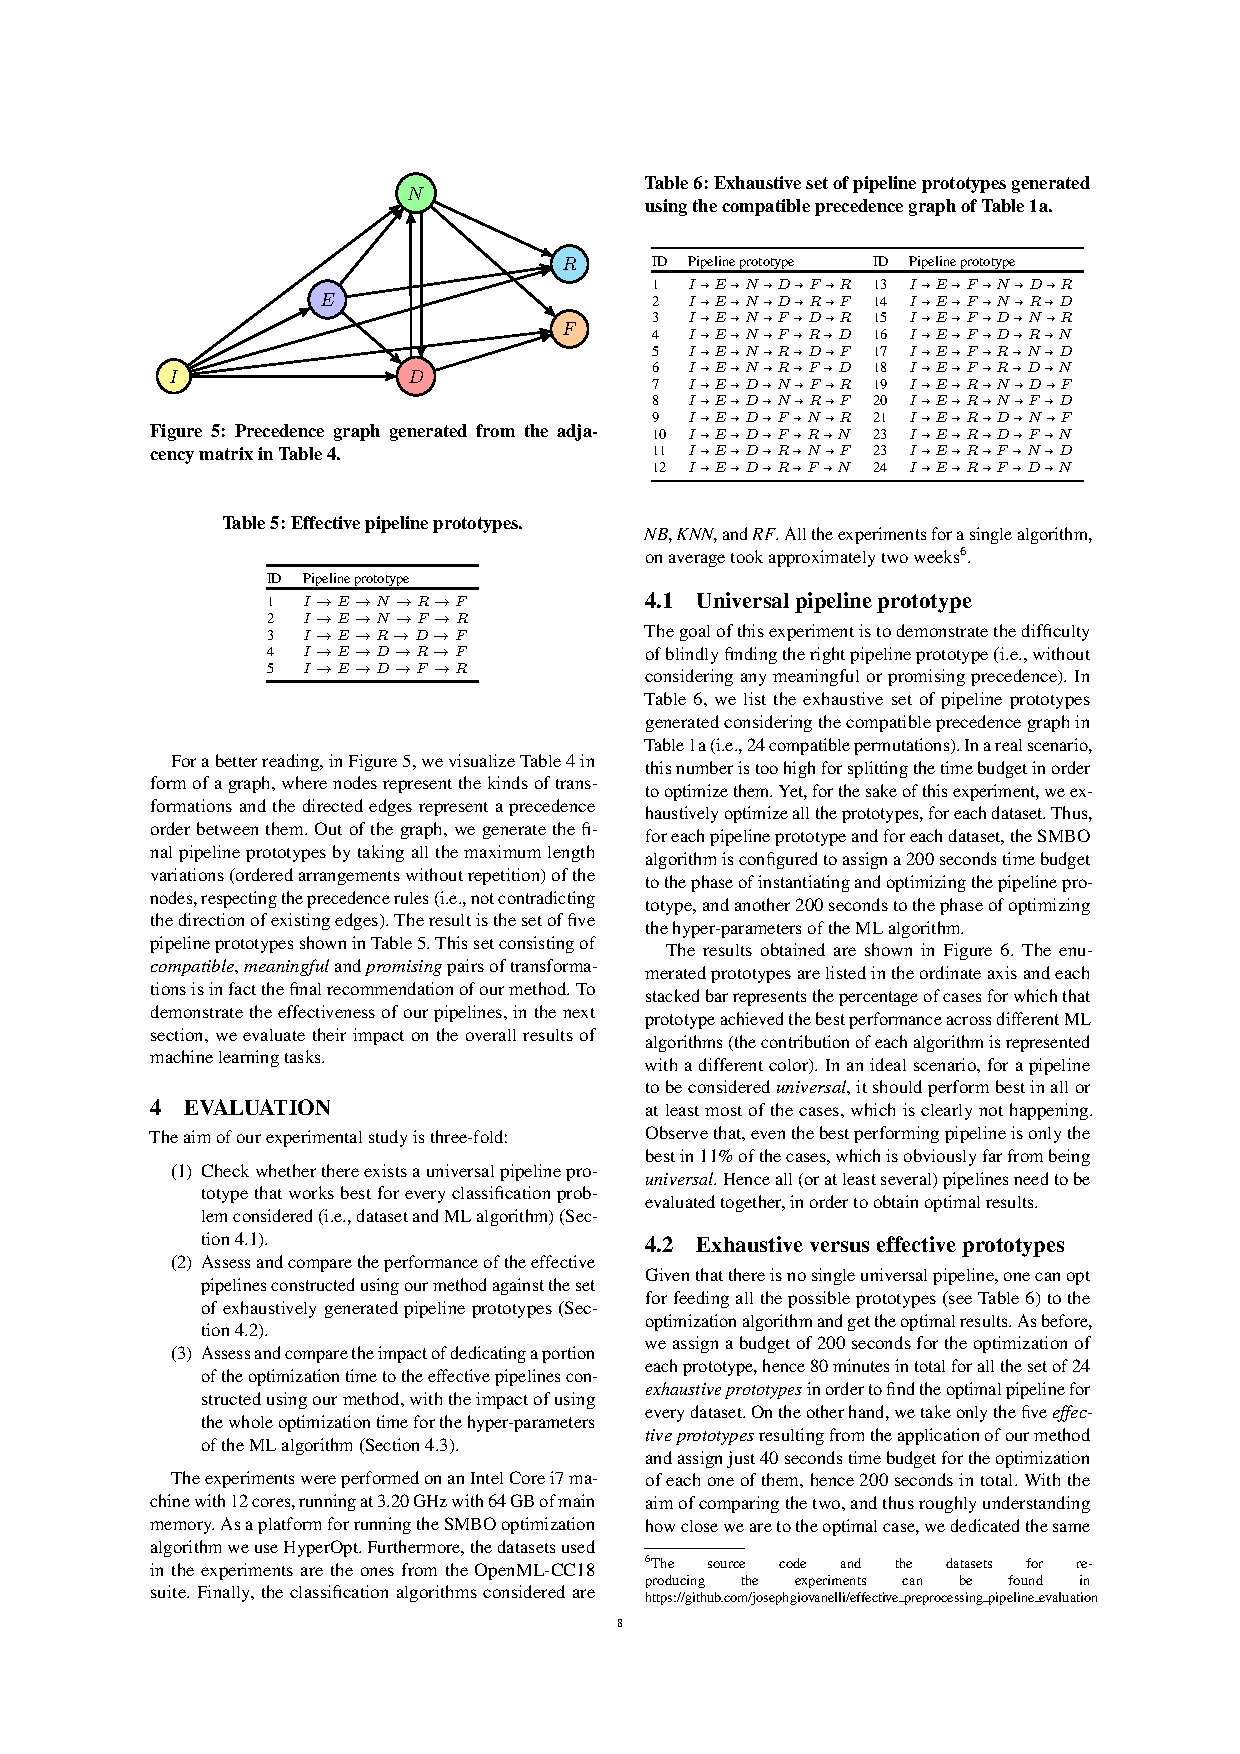
\includegraphics[clip, trim=2.5cm 23cm 10.5cm 2cm,width=0.5\textwidth]{part-automl/chapter-supervised/img/graph.pdf}
    %\label{fig:precedence-graph}
	%\caption{}
}{%
  	\caption{Precedence graph generated from Table~\ref{tbl:rules-union}. $E$ - Encoding; $N$ - Normalization; $D$ - Discretization; $I$ - Imputation; $R$ - Rebalancing; $F$ - Feature Engineering. }
}
\capbtabbox{%
\begin{tabular}{@{}ll}
			\toprule
			ID& Pipeline prototype                                             \\ \toprule
			1&{\color[HTML]{000000} $I\rightarrow E\rightarrow N \rightarrow R\rightarrow F$} \\
			2&{\color[HTML]{000000} $I\rightarrow E\rightarrow N \rightarrow F\rightarrow R$} \\
			3&{\color[HTML]{000000} $I\rightarrow E\rightarrow R \rightarrow D\rightarrow F$} \\
			4&{\color[HTML]{000000} $I\rightarrow E\rightarrow D \rightarrow R\rightarrow F$} \\
			5&{\color[HTML]{000000} $I\rightarrow E\rightarrow D \rightarrow F\rightarrow R$} \\
			\bottomrule
		\end{tabular}
}{%
  	\caption{Effective pipeline prototypes generated from Figure~6. $E$ - Encoding; $N$ - Normalization; $D$ - Discretization; $I$ - Imputation; $R$ - Rebalancing; $F$ - Feature Engineering.
	}
}
\end{floatrow}
%\besim{@Joseph, I think putting Figure 7 and Table 6 in the same row is nicer, because they are related. But with the package I am using, it seems I cannot label the table, and thus cannot refer to it in the text (an easy solution is to hardcode the reference:), as I did for the moment). Maybe you can check for another package or try to fix it. Just don't spend too much time, I think for the moment we can leave it hard-coded.}

\end{figure}



\iffalse

\begin{figure}[t]
	\centering
	
	\begin{tikzpicture}[]
	%% Draw system flow diagram
	\begin{scope}[xshift=10.5cm,yshift=-5cm,thick,
	node distance=1.0cm,on grid,>=stealth',
	block/.style={rectangle,draw,fill=cyan!20},
	vertex/.style={circle,draw,fill=orange!40},
	i/.style={circle,draw,fill=yellow!40},
	e/.style={circle,draw,fill=blue!25},
	f/.style={circle,draw,fill=orange!40},
	r/.style={circle,draw,fill=cyan!40},
	n/.style={circle,draw,fill=green!40},
	d/.style={circle,draw,fill=red!40}]
	decision/.style={diamond,draw,fill=white!40}]
	%layer0
	\node [i]	 (ti0) {$I$};
	\node [e]	 (te0)	[right=of ti0,xshift=1.6cm,yshift=1.3cm]	{$E$} edge [<-] (ti0);
	\node [n]	 (tn0)	[right=of te0,xshift=0.5cm,yshift=1.8cm]	{$N$} edge [<-] (te0);
	\node [d]	 (td0)	[right=of te0,xshift=0.5cm,yshift=-1.3cm]	{$D$} edge [<-] (te0);
	
	\node [r]	 (tr0)	[right=of tn0,xshift=1.6cm,yshift=-1.2cm]	{$R$} edge [<-] (tn0);
	
	\node [f]	 (tf0)	[right=of tn0,xshift=1.6cm,yshift=-2.3cm]	{$F$} edge [<-] (tn0);
	
	\path [->,draw,thick] (ti0) -- (tn0); 
	\path [->,draw,thick] (ti0) -- (tr0);
	\path [->,draw,thick] (ti0) -- (tf0);
	\path [->,draw,thick] (ti0) -- (td0);
	\path [->,draw,thick] (te0) -- (tr0);
	\path [->,draw,thick] (ti0) -- (tf0);
	\path [->,draw,thick] (td0) -- (tf0);
	\path [->,draw,thick] (tn0.285) -- (td0.75);
	\path [->,draw,thick] (td0.105) -- (tn0.255);
	\end{scope}
	\end{tikzpicture}
	\caption{Precedence graph generated from Table~\ref{tbl:rules-union}. $E$ - Encoding; $N$ - Normalization; $D$ - Discretization; $I$ - Imputation; $R$ - Rebalancing; $F$ - Feature Engineering.
	}
	\label{fig:precedence-graph}
\end{figure}


\begin{table}[t]
	\caption{Effective pipeline prototypes generated from Figure~6%\ref{fig:precedence-graph}
	. $E$ - Encoding; $N$ - Normalization; $D$ - Discretization; $I$ - Imputation; $R$ - Rebalancing; $F$ - Feature Engineering.
	}
	\footnotesize
	\label{tbl:effective-pipelines}
	\begin{center}
		\begin{tabular}{@{}ll}
			\toprule
			ID& Pipeline prototype                                             \\ \toprule
			1&{\color[HTML]{000000} $I\rightarrow E\rightarrow N \rightarrow R\rightarrow F$} \\
			2&{\color[HTML]{000000} $I\rightarrow E\rightarrow N \rightarrow F\rightarrow R$} \\
			3&{\color[HTML]{000000} $I\rightarrow E\rightarrow R \rightarrow D\rightarrow F$} \\
			4&{\color[HTML]{000000} $I\rightarrow E\rightarrow D \rightarrow R\rightarrow F$} \\
			5&{\color[HTML]{000000} $I\rightarrow E\rightarrow D \rightarrow F\rightarrow R$} \\
			\bottomrule
		\end{tabular}
	\end{center}
\end{table}
\fi

\end{example}
%\subsection{Pipeline prototype construction}
\subsubsection{Effective pipeline prototypes}
\label{ssec:composition}
In this task we foresee the composition of the previously defined rules (i.e., for the pairs of transformations), to generate the final set of rules that would allow to compose longer chains --- consisting of more than two transformations. This is when we resolve the inconsistencies and also define precedences for the pairs of transformations that may not have any precedence defined already --- in that case, we basically take into account all the permutations. This step allows to finally generate the possible effective pipeline prototypes. 

\begin{example}
To generate the final pipeline prototypes, in this step we combine all the matrices generated by the previous steps. That is, we take the union of the edges (represented by \texttt{1}'s) from the matrices in Table~\ref{tbl:rules} (a,b,c), and create a new final adjacency matrix, shown in Table~\ref{tbl:rules-union}. This is the matrix that will allow us to generate the final effective pipeline prototypes. 

Observing the table, one can realize that for pairs $\{F,R\}$ and $\{R,D\}$, no precedence edges exist. This means that these pairs are somewhat equally relevant from either direction (any order), and thus when generating the final prototypes, both options should appear.

For a better reading, in Figure~6, we visualize Table~\ref{tbl:rules-union} in form of a graph, where nodes represent the kinds of transformations and the directed edges represent a precedence order between them.
Out of the graph, we generate the final pipeline prototypes by taking all the maximum length variations (ordered arrangements without repetition) of the nodes, respecting the precedence rules (i.e., not contradicting the direction of existing edges). The result is the set of five pipeline prototypes shown in Table 6. This set consisting of \textit{compatible}, \textit{meaningful} and \textit{promising} pairs of transformations is the set of recommended \textit{effective pipeline prototypes}.
\end{example}

\color{black}
\subsubsection{Meta-learning rules}
\label{ssec:meta-learning}
Once the pipeline prototype is constructed, that is, the order between the kinds of transformations is defined, what follows is the instantiation of transformations with the physical operators. For that, one can rely completely on the optimization algorithm, and let the algorithm choose the right operators. However, given the way optimization algorithms work (e.g., SMBO) --- successively finding better and better instantiations, there is a cold-start problem, where in the beginning, the algorithm does not have enough information in order to come up with the most promising initial instantiations, and a wrong choice may affect the optimization process. 
\paragraph{Exploratory analysis}
Given the availability of the experimental SMBO executions (executed in an exhaustive manner, considering all the pipeline prototypes), one can perform an exploratory analysis with the aim of removing useless prototypes, pipelines or operators. Hence, further tweaking the search space. In particular, starting from the highest level, that of prototypes, then going to the physical pipelines, and finally to the actual operators inside the pipeline, one can analyze if:

\begin{itemize}
    \item there exist some combination of transformations in the form of prototypes (see Table~\ref{tbl:pipeline-enumeration} for the exhaustive list of prototypes), that are generally useless (i.e., in terms of their impact to the final accuracy), and thus can be discarded a priori in order to reduce the search space, 
    \item there are some physical pipelines that are consistently chosen more often than others by the optimization algorithm, meaning that they are more useful than others,
    \item within the physical pipelines, some transformations are chosen more often than others, meaning that they provide more positive impact. 
    \end{itemize}

\begin{example}
We performed the above-mentioned analysis to our use case, but it did not lead to any conclusive or significant results. In particular, as shown in Figure~\ref{fig:prototypes-impact}, we could not find any useless prototypes --- not positively impacting the final accuracy, that could be discarded a priori from the potential list of prototypes.
Actually, as we will show in Section~\ref{ssec:eval-universal-pipeline}, all of them lead to the best in one case or another, which does not mean the epsilon improvement some provide is worth the search cost you incur in considering them (but this more in-depth analysis is done later).
Next, as shown in Figure~\ref{fig:pipeline-frequency}, there were no physical pipelines shown to be more useful --- hence more often selected, than others. Even if $N \rightarrow R$ is clearly above, it barely reaches 30\% in KNN.
 Finally, observing Figure~\ref{fig:transformation-frequency}, it is clear that some kinds of transformations are chosen more often, but looking closely (i.e., the shaded bars), it is not clear which operator brings more benefit. For instance, Normalization is present in 90\% of the pipelines, but it is not easy to distinguish which kind of Normalization (i.e., actual operator) is more beneficial.
For this, we need more complex rules or guidelines that may help in finding the right operator to use. 
\end{example}

\begin{figure*}[!t]
	\centering
	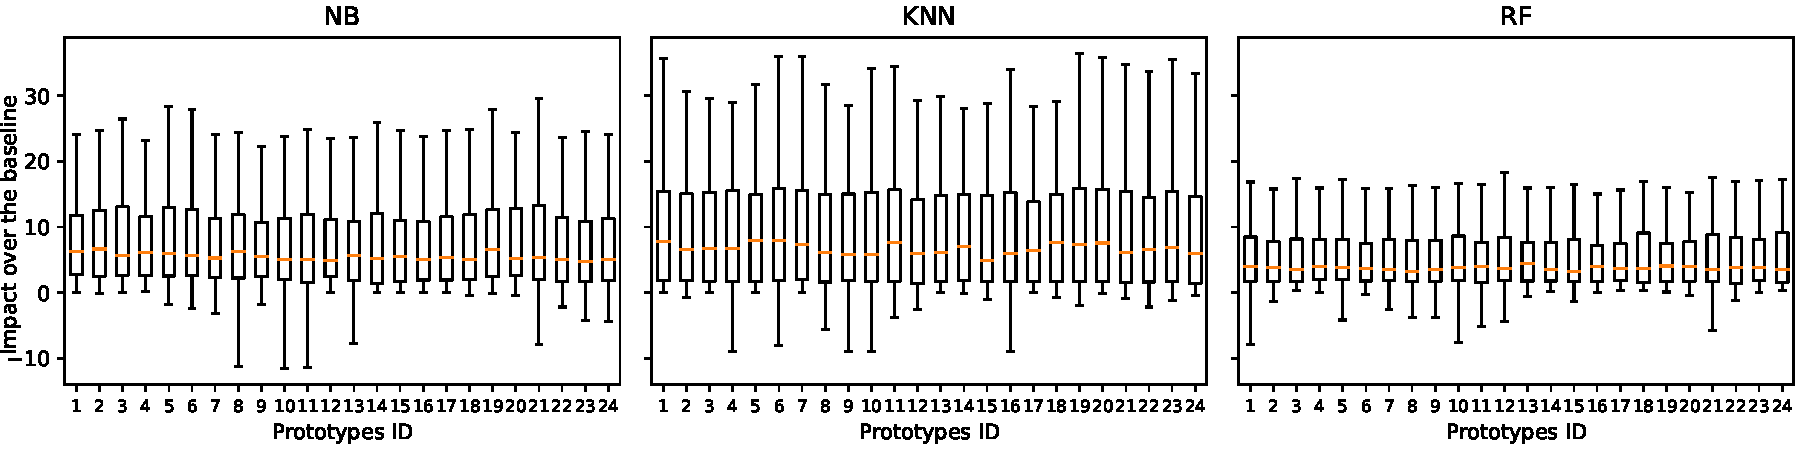
\includegraphics[width=1.0\textwidth]{part-automl/chapter-supervised/img/prototypes_impact.pdf}
	\caption{The impact of the different pipeline prototypes over the baseline (i.e., when no transformation is applied).}
	\label{fig:prototypes-impact}
	%\besim{The x label, I would change it to 'Prototype ID'}
\end{figure*}

\begin{figure*}[!h]
	\centering
	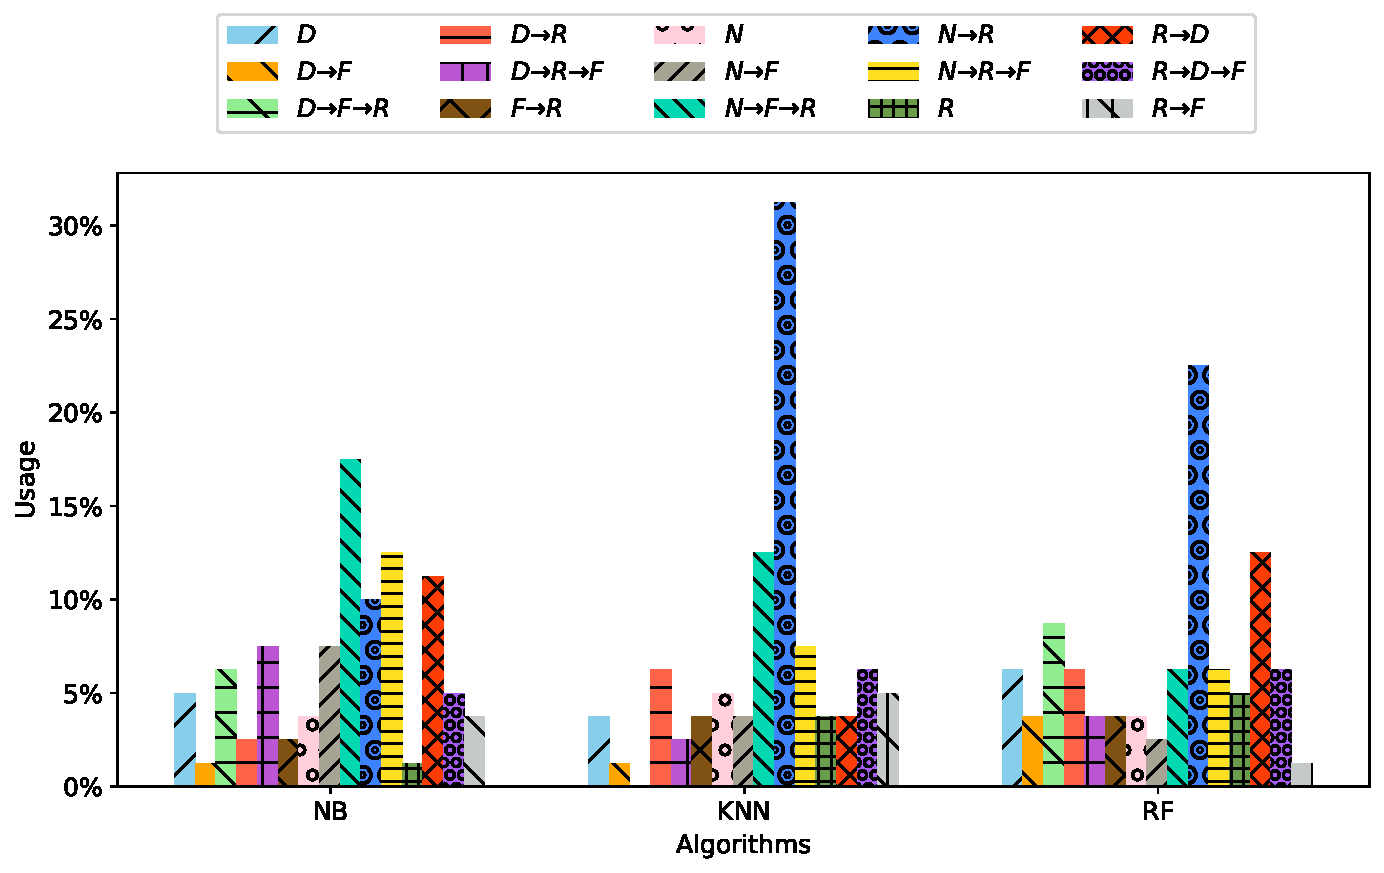
\includegraphics[width=1.0\textwidth]{part-automl/chapter-supervised/img/pp_pipeline_study2.pdf}
	\caption{Percentage of use of the different physical pipelines.}
	\label{fig:pipeline-frequency}
\end{figure*}

\begin{figure*}[!h]
	\centering
	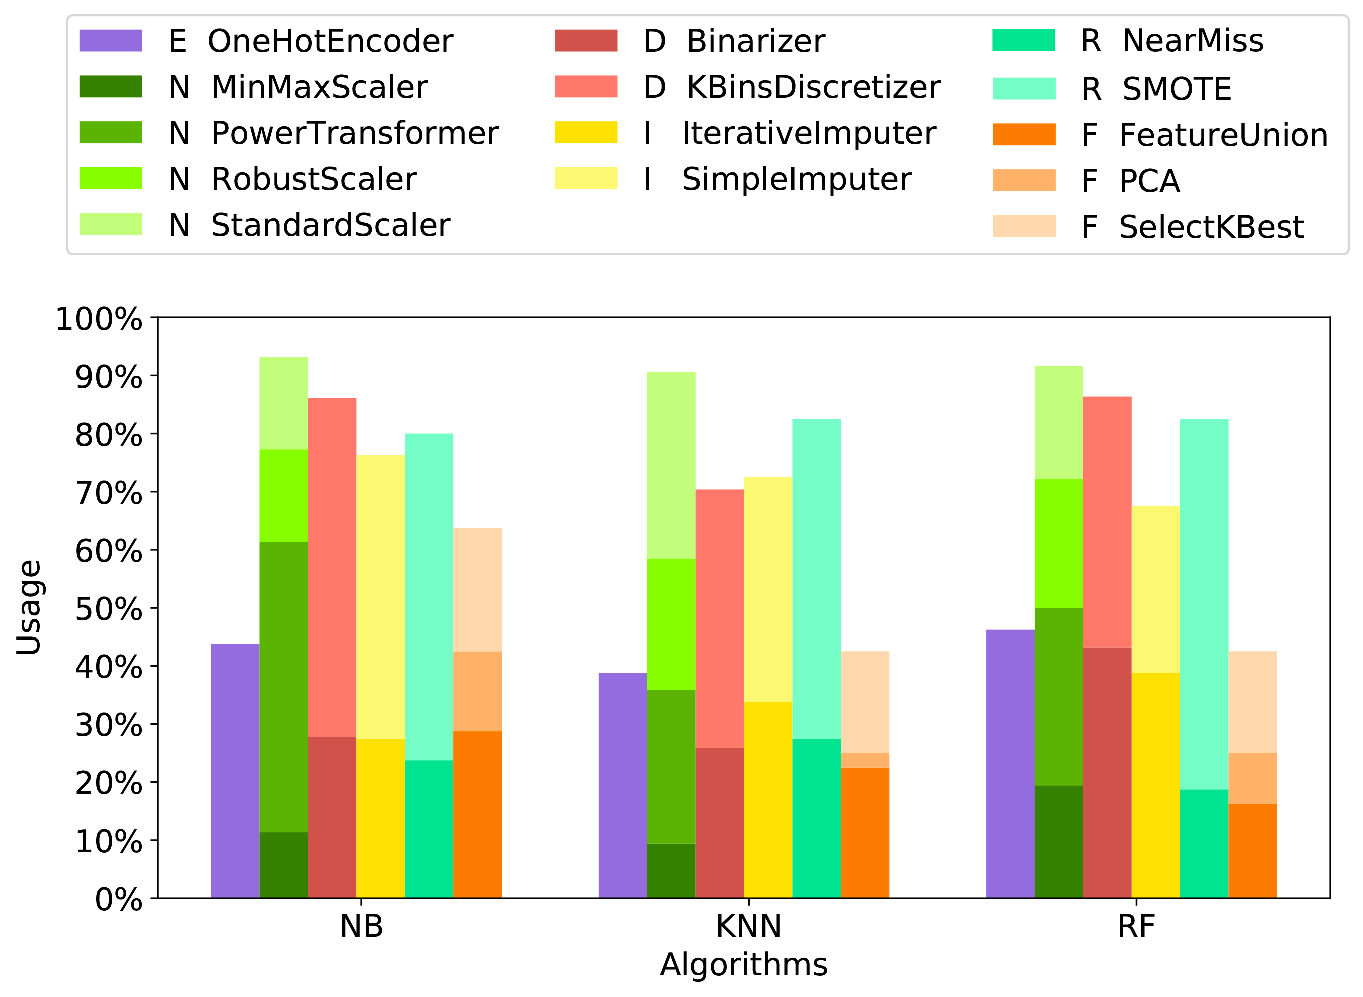
\includegraphics[width=0.7\textwidth]{part-automl/chapter-supervised/img/pp_pipeline_study_grouped.pdf}
	\caption{Percentage of use of a transformation in a physical pipeline.}
	\label{fig:transformation-frequency}
	%\besim{In the legend, is it easy to put each kind of transformation in separate columns?}
\end{figure*}

\subsubsection{Meta-learning}
\color{black}
To mitigate the red cold-start problem, we propose to perform meta-learning (shown in Figure~\ref{fig:methodology}), where we intend to use the knowledge extracted from historical data in order to devise rules that may help the optimization algorithm in its initial phase. 
Meta-learning is the process of `learning on top of learning', or learning a model using historical data from ML experiments. Traditionally, it has been used for predicting the performance (e.g., predictive accuracy) of an algorithm on a given dataset. That is, given some historical runs of the performance of classification algorithms over various datasets (i.e., meta-database: consisting of datasets characteristics as predictive variables and the performance of the classification algorithm as the response variable), one can learn a model (i.e., meta-model), that is able to predict the performance of a given classification algorithm on a new dataset~\cite{Brazdil04Book}. Lately, this technique has been extended in order to predict the impact of transformations over the performance of classification algorithms and thus rank transformations based on their impact~\cite{Bilalli17AMCS, presistant18CSI, presistant19DKE}. The same idea can be applied for learning the best operator for a given transformation.
That is, through meta-learning one can learn the intrinsic relationship between dataset characteristics and the operator performance, and thus come up with rules that are not obvious and are effective at the time of instantiating a transformation. 
The main idea is to build a model, that is able to predict the operator for a certain kind of transformation, given the meta-features extracted from the dataset considered for the optimization. This translates to answering the following question: ``given that we know the dataset characteristics and having selected a certain kind of transformation (e.g., missing value imputation), what is the optimal physical algorithm (see Table~\ref{tbl:transformations}) we need to select, to obtain the highest improvement possible in terms of classification accuracy (i.e., when the classification algorithm is applied over the transformed dataset)?".  In particular, the model can generate a set of complementary rules that help in the optimization, providing a good starting instantiation for some of the transformations in the prototype.

To train the model we need a meta-dataset that can be  (i) generated through optimization algorithms (e.g., SMBO executions), (ii) generated manually through simple evaluations of classification algorithms over transformed datasets, or (iii) assumed already given (e.g., OpenML). 

Given a meta-dataset, we propose to learn to predict the best instantiation (operator) for a given transformation, where among the classes we can include the class \texttt{None} too. This means that one of the possible predictions is to not instantiate a transformation at all, hence remove it from the pipeline.

\begin{example}
Our training dataset (sometimes referred to as `meta-database' or `meta-dataset') for the meta-learning is compiled through SMBO runs on the OpenML datasets (see Section~\ref{ssec:rules-learned:algorithm}). That is, we first extract the dataset characteristics/profiles (i.e., number of features, number of instances, number of missing values, etc), and then by applying SMBO optimization, on classification algorithms and pre-processing pipelines (as explained in Section~\ref{ssec:composition}), for each dataset, we retrieve the evaluations (i.e., predictive accuracy) of the algorithms over the optimized pipelines. This gives us the presumably optimal physical pipelines and their impact on the accuracy of the learning algorithms for each dataset at hand. Given such information, our aim is to now save time and improve the instantiation of the operators for each transformation considered in the prototype. 

We trained several different Conditional Inference Trees \cite{ctree} because they produce models that can be easily read and interpreted.
Specifically, the independence of each variable (meta-features in our case) with the class (operator of a specific transformation) is tested through a statistical test. 
The split is made on the variable with the lowest p-value. 
We report the p-value too, so that it can be seen how strong the association is (i.e., why that variable was chosen).
We stick with the p-value threshold of 0.05, and devise a rule from any branch of the tree that is within the threshold. In the following, we describe the rules obtained within the selected significance threshold.

\textbf{Rules for Feature Engineering}. The available operators in Scikit-learn for Feature Engineering (see Table~\ref{tbl:transformations}) are: \texttt{PCA} (Principal Component Analysis), \texttt{Feature Selection} (Select K Best), \texttt{Both} (PCA + Select K Best), and \texttt{None}. The tree generated for the Feature Engineering transformation is shown in Figure~\ref{fig:features-meta-learning:feature-engineering}. The leaves show the selected operator frequency. For the sake of simplicity, we do not consider the union of PCA and Select K Best as an operator per se, instead we distribute that contribution to the two operators that compose it.
Observe that there is a strong correlation between the Feature Engineering operator and the entropy of the class attribute.
Indeed, such a meta-feature achieved a p-value smaller than 0.001.
We can clearly read that if the Class Entropy is low, then \texttt{Feature Selection} is way more chosen than the other options (see Node 2).
Recall that the entropy of an attribute is a measure of how much disorder there is among its instances.
The less is that value, the easier is the classification problem.
As a consequence, it is reasonable to think that the easier the classification problem is, the more likely is the fact that the class can be described by a low number of features.
Hence, the \texttt{Feature Selection} technique can be successfully applied.
Conversely, Node 5 shows that, when the Class Entropy is high, it is better to not apply any Feature Engineering operator.
As a matter of fact, a high value of Class Entropy involves a high number of classes and/or few instances per class, hence a really difficult problem.
In such cases, reducing the dimensionality of the dataset does not lead to any improvement.
Finally, when the Class Entropy is in between, there is no clear winner, and thus other non-obvious factors may affect the choice of the operator.

\textbf{Rules for Rebalancing}. As for Rebalancing, the operators considered from the imblearn\footnote{\url{https://pypi.org/project/imbalanced-learn}} library are: \texttt{Near Miss}, \texttt{SMOTE}, and \texttt{None}. %\joseph{the rebalance implementations are of actually from imblearn (imbalanced-learn)}
The first is an undersampling algorithm which randomly eliminates the samples from the larger class.
Instead, the second is an oversampling technique that creates samples of the minority class, as a linear combination of them.
As shown in Figure~\ref{fig:features-meta-learning:rebalancing}, the meta-feature Majority Class Percentage has a p-value of 0.014.
This can be read as, in case of an unbalanced class problem (i.e., Node 3: Majority Class Percentage greater than 56), an oversampling of the minority class(es) is preferred to a downsampling of the majority one(s).
However, when the Majority Class Percentage is smaller than 56\%, the situation is not that clear, and there is no technique that is applied significantly more often than the rest; they are close to each other.
Therefore, it is difficult to understand which problems (which dataset characteristics do they have) belong to Node 2.
In summary, when the majority class has no more than 56\% , it implies that it is an unbalanced class, and as mentioned above, SMBO tends to choose the same operator. However, when the majority class has less than 56\%, it may imply that: (i) there are just two classes and the problem counts as a balanced problem, so no operator needs to be applied, or (ii) it is a multi-class problem, and thus there is no clear winner in terms of operators. 
\end{example}


\subsection{Prototype instantiation}

The prototypes from the top flow and the meta-lerning rules from the bottom flow (if the optimization framework permits), are finally fed to the final step which deals with the instantiation and optimization of the prototypes. In this task we run an optimization algorithm that is executed until an optimal pipeline is found.

\begin{example}
 In our final execution, we run SMBO to find a suitable instantiation for the suggested prototypes. The simple but not obvious meta-learning rules, even though not included in our final execution, because of the implementation considered (i.e., HyperOpt), can potentially be used to ease the cold-start problem. 
\end{example}

\begin{figure*}[!h]
	\centering
	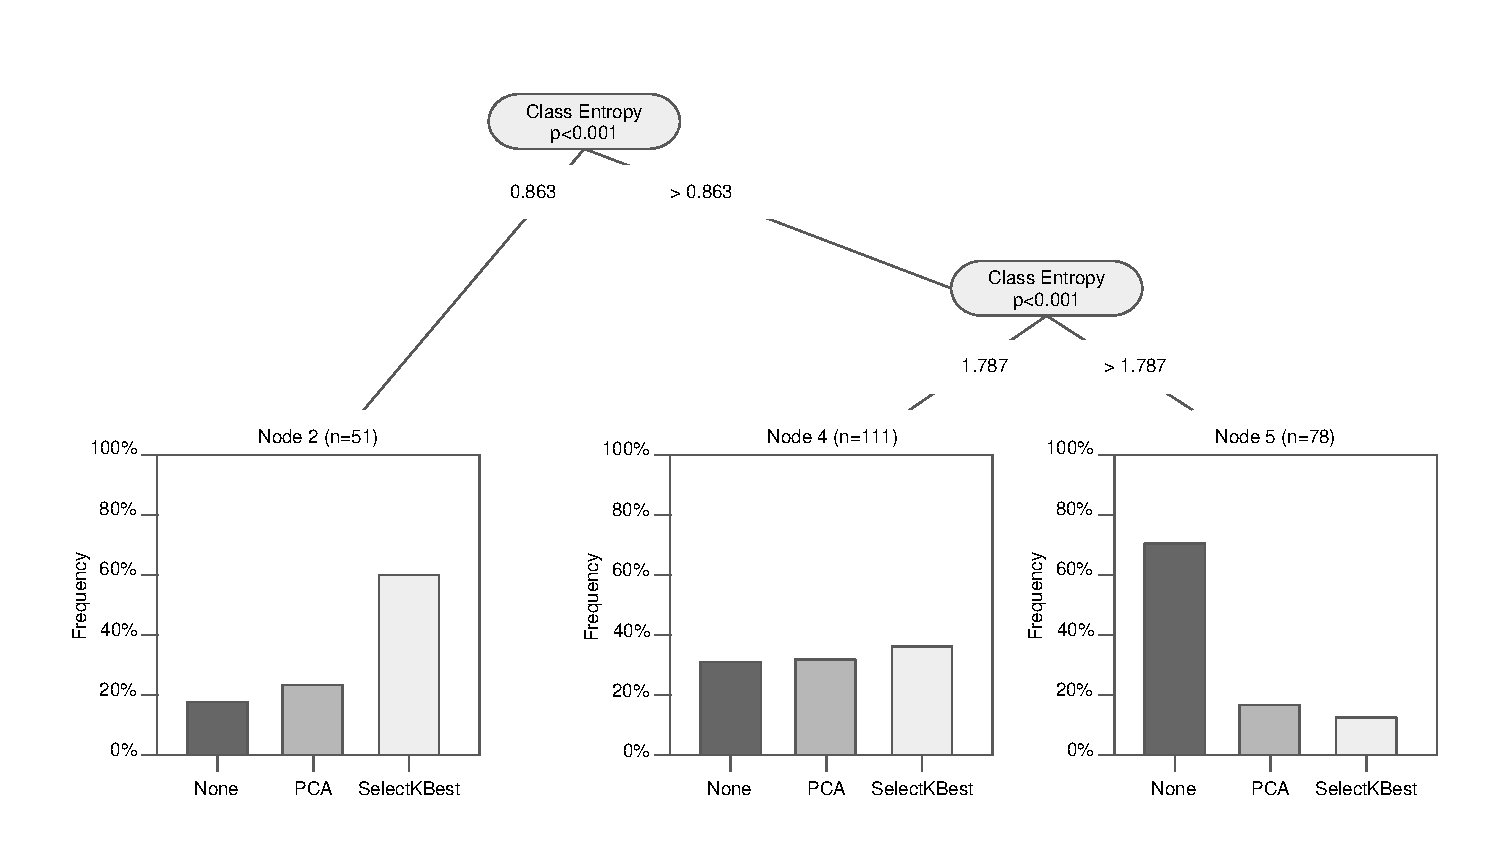
\includegraphics[clip, trim=1.0cm 0.4cm 1cm 1cm,width=1\textwidth]{part-automl/chapter-supervised/img/tree-FE.pdf}
	\caption{Conditional Inference Tree built for the \textit{Features Engineering} transformation.}
	\label{fig:features-meta-learning:feature-engineering}
	%\joseph{\\
    %Node 2: \{None: 0.18, PCA: 0.22, SelectKBest: 0.6\} \\
    %Node 4: \{None: 0.31, PCA: 0.32, SelectKBest: 0.36\} \\
    %Node 5: \{None: 0.7, PCA: 0.17, SelectKBest: 0.13\}
	%}
\end{figure*}

\begin{figure*}[!h]
	\centering
	%left, lower, right, upper
	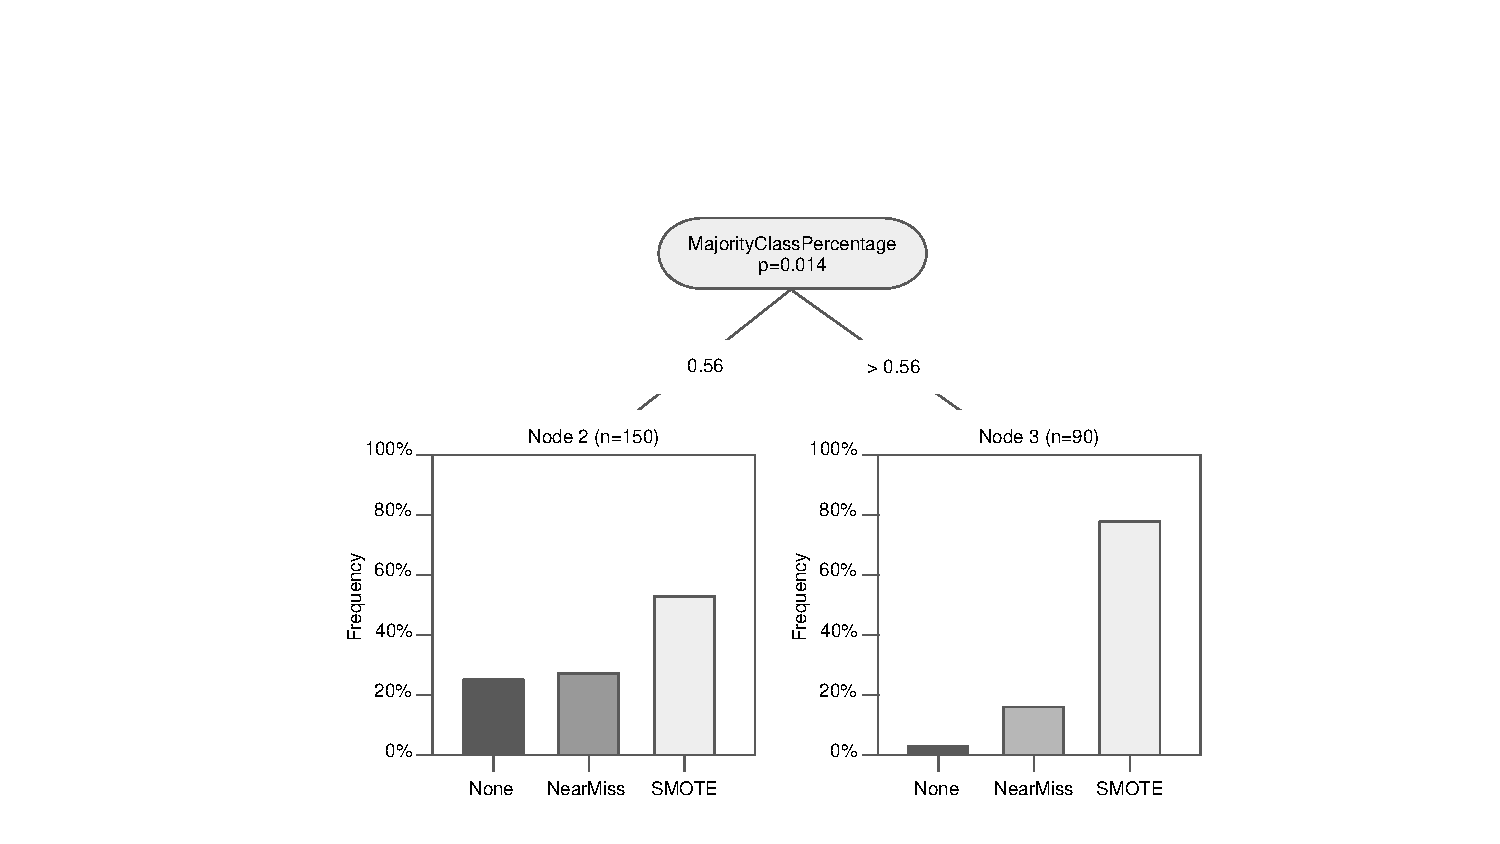
\includegraphics[clip, trim=5.8cm 0.4cm 5.05cm 3.5cm,width=0.65\textwidth]{part-automl/chapter-supervised/img/tree-RE.pdf}
	\caption{Conditional Inference Tree built for the \textit{Rebalancing} transformation.}
	\label{fig:features-meta-learning:rebalancing}
	%\besim{@jospeh, Sorry, I have the source (corel draw), but it complains about the version and does not open it. Do you think you can add the labels on top of the pdf? I think it should be Arial the font.}
	%\joseph{\\
    %Node 2: \{None: 0.25, NearMiss: 0.27, SMOTE: 0.48\} \\
    %Node 3: \{None: 0.07, NearMiss: 0.16, SMOTE: 0.77\}}
    %\besim{It would be better to put this just below Figure 11, but I didn't manage!}
\end{figure*}

%In our recent future work we aim to extend HyperOpt with the functionality of incorporating mechanisms that ease the cold start problem. The technique of using meta-learning for the cold-start problem has for instance been applied in \cite{Feurer15AAAI}, however the overall method lacks the initial part of finding promising pipeline prototypes (i.e., works over single transformations), meaning that the instantiation via meta-learning may occur in the wrong place (not the optimal prototype), resulting into a solution that is a local optimum. 